\documentclass{jpconf}

% graphics packages
\usepackage{graphicx}
\usepackage{stackengine}
\usepackage{caption}
\usepackage{subcaption}
\usepackage{float}
\usepackage{placeins}

% algorithm packages
%\usepackage{algpseudocode}
%\usepackage{algorithm}
\usepackage{amsmath}

% symbols
\usepackage{gensymb}

% reference packages
\usepackage[hidelinks]{hyperref}
\usepackage{cleveref}
\usepackage{url}
\usepackage{hypcap} % fix the links

% formatting packages
\usepackage{enumitem}
\usepackage{flafter}
\usepackage{booktabs}
\usepackage[letterpaper, margin=1in]{geometry}
\usepackage[flushleft]{threeparttable}

% paths
\graphicspath{{./final_images/}}

% editing packages
\usepackage{todonotes}

\begin{document}

\title{Wake Expansion Continuation: \large{Multi-modality reduction in the wind farm layout optimization problem}}

\author{J~J~Thomas, S~McOmber, and A~Ning}
\address{Department of Mechanical Engineering,
Brigham Young University, Provo, Utah, USA}
\ead{jaredthomas@byu.edu}

\begin{abstract}
	This paper presents a process using an approach related to  continuation optimization methods for reducing multi-modality in the wind farm layout optimization problem, referred to as Wake Expansion Continuation (WEC). The reduction in multi-modality is achieved by starting with an increased wake spread while maintaining normal velocity deficits at the center of the wakes, and then reducing the wake spread for each of a series of optimization runs until the standard wake spread is used. WEC was applied and shown effective with two different wake models. Four optimization case studies were tested with a gradient-based optimization method and a gradient-free optimization method. Results using WEC show a significant improvement in mean optimized annual energy production (AEP) compared to optimization without WEC for all test cases. The gradient-free optimization algorithm found less optimal results on average for all cases than the gradient-based algorithm with WEC. WEC was also applied to the gradient-free algorithm for one case study with significantly improved results, but the improvement was more significant when WEC was applied to a gradient-based algorithm.
\end{abstract}

\section{Introduction}

The difficulty of solving the wind farm layout optimization (WFLO) problem is primarily due to the large number of variables and constraints required for realistic problems and the multi-modal nature of the problem's design space. Gradient-free optimization methods are the most common methods used to solve the WFLO problem. However, gradient-free methods have been shown to have reduced performance with high dimensional problems \cite{rios2013-grad-free-comparison}. The WFLO problem scales quickly to high dimensions as the number of turbines is increased. Gradient-based optimization methods are well suited for high dimensional problems. Gradient-based methods are not widely used for WFLO problems because they are highly susceptible to local optima \cite{acero2014}, but they are gaining interest due to their relatively low computational cost and their ability to efficiently handle many variables and constraints. Gradient-based methods have been shown to find good solutions to WFLO problems \cite{fleming2015, guirguis2016, gebraad2017-Maximization-Annual}.  

Many techniques have been presented to make the WFLO problem more tractable, including discretization, multi-start, re-parameterization, and hybrid approaches. Discretization techniques, used with gradient-free methods, attempt to simplify the problem by reducing the number of possible solutions \cite{mosetti1994, grady2005}. Through discretization, the number of possible turbine locations within a wind farm can be reduced from infinite to something on the order of hundreds of locations. However, discretization disregards any locations that are not pre-selected, and can thus preclude this approach from finding even a local optimum. It is also possible that constraints on variables other than position may render the discretized optimization problem intractable. Multi-start approaches involve running many optimizations of one problem with different starting points \cite{gonzalez2014}. This approach reduces the sensitivity of gradient-based optimization methods to local optima. Re-parameterization approaches seek to reduce the complexity of the problem by defining the wind farm with just a few variables, such as row spacing, column spacing, grid rotation, etc.~as done in \cite{stanley2020}. Hybrid approaches combine gradient-based and gradient-free algorithms iteratively \cite{rethore2014,graf2016, mittal2017}, and, depending on the problem size, can yield comparable results to multi-start approaches \cite{rethore2014}. While each of these techniques yield improved results, there is still need for further improvement because current methods have a wide spread in the quality of results, are highly dependent on starting locations, artificially limit the design space, and/or cannot be applied in realistic wind farm optimization scenarios. These limitations indicate that there is need for better optimization methods that avoid local optima, whether real or imposed by the approach itself.

Current methods seek to avoid local optima by searching the existing design space more broadly. Broadly searching the design space becomes intractable for large optimization problems with many variables and constraints. To avoid local optima without requiring a broad search of the design space, we propose a process for use with gradient-based optimization algorithms that temporarily reduces the number and magnitude of local optima using a continuation optimization approach similar to the Gaussian continuation method discussed in \cite{mobahi2015}. While the referenced Gaussian continuation optimization method uses an approximation, or surrogate, of the simulation model, our proposed method takes advantages of the model parameters directly. 

The two primary characteristics that simple wake models seek to capture are wake diameter and velocity deficit. These characteristics in turn largely determine the shape of the wind farm layout design space. The fluctuations of wind speed as turbines move in and out of the wakes during optimization are primarily responsible for the multi-modal nature of the WFLO problem. 

During optimization, the spaces between wakes translate to locally optimal locations for turbines. However, it is often the case that there are more optimal turbine locations that are not found by the optimizer because the turbines are effectively stuck in locally optimal locations. In this paper we propose a method designed to overcome the problem of local optima caused by wind speed fluctuations as wind turbines move in and out of the wakes. We reduce the impact of local optima by widening and combining wake regions without altering individual wake-center deficits. We then run a series of optimizations with increasingly realistic wake distributions until we get back to the original model. We will refer to the new method as Wake Expansion Continuation, or WEC. 

In the following sections, we will: present an overview of WEC (\cref{sec:introwec}), introduce the simulation models used to study WEC (\cref{sec:models}), demonstrate how to apply WEC to existing models (\cref{sec:application}), provide a series of wind farm layout optimization case studies for comparing optimization methods (\cref{sec:casestudies}), give some details on the computational environment used in our studies (\cref{sec:computation}), discuss how we tuned the various methods for our case studies (\cref{sec:tuning}), present and discuss the results of the case studies (\cref{sec:results}), and provide concluding comments (\cref{sec:conclusion}).

\section{Introduction to the Wake Expansion Continuation}\label{sec:introwec}

The WEC method is somewhat analogous to Gaussian continuation optimization. In Gaussian continuation optimization, the design space is approximated using a series of Gaussian radial basis functions. When optimization is performed, the standard deviations of the radial basis functions starts at a relatively high value and slowly decreases until the original standard deviation is reached \cite{mobahi2015}. Increasing the standard deviation of the basis functions has the effect of causing the various basis functions to blend in to each other, effectively removing the local optima and providing a relatively convex design space to the optimization algorithm. Slowly returning the standard deviation to the original value allows the optimization algorithm to adjust for any shift in the global optimum due to the blending of the basis functions and avoid local optima. 

WEC works in a manner similar to Gaussian continuation optimization, except that because wind turbine wakes are roughly Gaussian-shaped, the Gaussian basis functions are built in to the model directly rather than used to approximate the model. Other key differences are that the basis functions in WEC are not radial, and that the Gaussian functions in the wind farm model change location during the WFLO. Because of these last two differences, we cannot guarantee that WEC will converge to the global optimum. However, the use of the WEC method does improve WFLO results. We have presented a preliminary study of the WEC method showing significant benefit in \cite{thomas2018-wec} and a follow-on study showing that optimization results using WEC were even more significant when re-calculated using large eddy simulations (LES) in \cite{thomas2019-les-validation}.

The WEC method can be explained in three basic steps. The first two steps are preparatory, and need only be performed once for each wake model:
\begin{enumerate}[label=\arabic*)]
	\item Determine how the wake diameter and wake deficit are controlled for the selected wake model.
    \item If necessary, introduce a factor to the model such that the wake diameter can be directly controlled without significantly altering the wake deficit in the center of the wake. If the model already provides such control then this step is not needed. Wake center is analogous to the mean of a Gaussian distribution. Wake deficit is analogous to the leading coefficient (parameter controlling curve height) of a Gaussian distribution. Wake spread is analogous to the standard deviation of a Gaussian distribution.  Keeping the wake deficit in the center of the wake constant, while changing the wake spread, mimics the behavior of increasing the standard deviation without changing the height of a Gaussian distribution as done in \cite{mobahi2015}. 
    \item Run a series of optimizations such that the wake diameter is larger than normal for the first optimization, and then reduces with each subsequent optimization until the wake spread is no longer altered from the original model. Each optimization after the first should be hot-started using the result of the previous optimization.
\end{enumerate}

The wakes create bumps in the design space. Gradient-based algorithms cannot get over the bumps on their own because they only like to go downhill. By spreading and combining the wakes (or bumps) the little bumps are covered up by the larger ones, reducing the number of individual bumps. A gradient-based optimization algorithm can then follow the slope of the conglomerate bump, over local optima in the real design space, and proceed to a better solution. Another way of thinking about this is that by spreading the wakes, more turbines see the influence of each wake, which provides more information to the gradient-based optimization algorithm about the design space through the Jacobian. 

To apply the wake expansion technique to the wind farm layout optimization problem, we need to determine the best way to expand the basis functions, or wake diameter in this case. We have investigated three ways of spreading the wake: (1) increasing the wake spreading angle (WEC-A), (2) multiplying the initial wake diameter (WEC-D), and (3) a hybrid of 2 and 3 that is accomplished by multiplying the wake diameter at an estimated point of far wake onset and allowing the wake to follow an angled line from the initial wake diameter to the expanded far wake diameter (WEC-H). The impact on the wake shape of each of these three methods of expanding the wake are shown in \cref{fig:wec-methods}.

\begin{figure}[h]
	\centering
	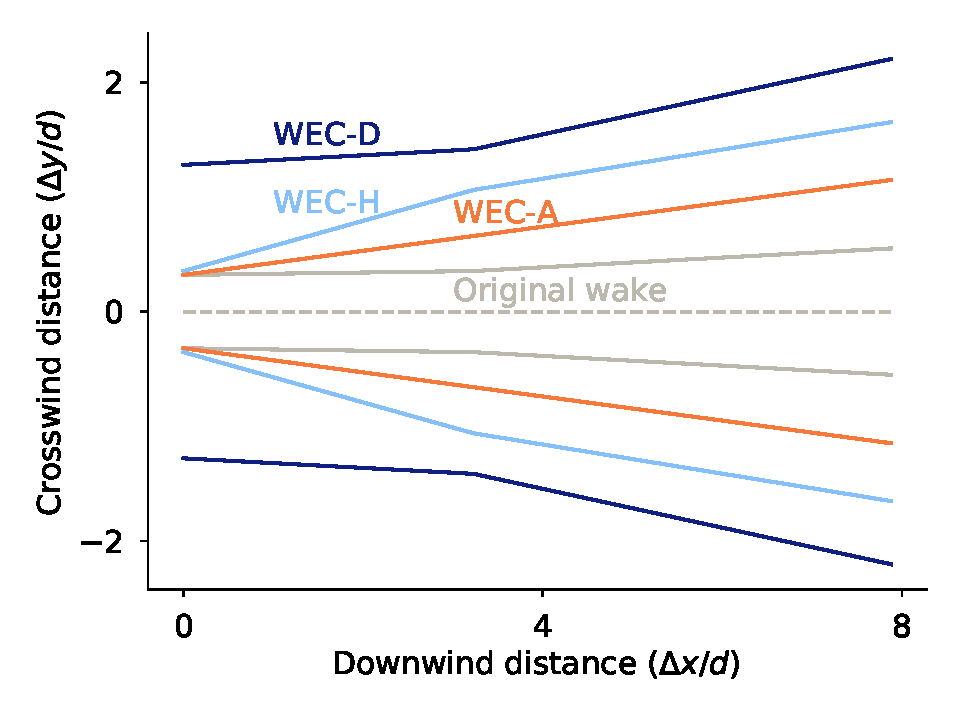
\includegraphics[width=0.6\textwidth,trim={0, 0, 0, 2.0}]{wec-methods}
	\caption{The impact on wake shape of expanding the wake by increasing the spreading angle (WEC-A), the diameter (WEC-D), or a downstream diameter that also changes the near wake spreading angle (WEC-H). The relative amount of expansion in the figure is for convenience in comparing the WEC methods. The actual amount of expansion is variable for all methods.}
	\label{fig:wec-methods}
\end{figure}

\section{Simulation Models}\label{sec:models}
Because of the general nature of the proposed method, it can be applied to any wake models where the wake center deficit and wake spread can be controlled independently. In this study we have applied WEC to the 2016 version of the Bastankhah and Port\'e-Agel wake model \cite{bastankhah2016}, which we will refer to as the Bastankhah model, and the cosine version of the Jensen wake model \cite{jensen1983}, which we will refer to as the Jensen cosine model. We also used various other models necessary for combining wakes and calculating wind farm AEP.

\subsection{The Bastankhah Wake Model}
In the Bastankhah wake model, two primary characteristics of the wakes, wake deficit and wake diameter, are particularly easy to isolate. This, along with the smoothness and differentiability of the model, make it a good example for demonstrating WEC. We used the Bastankhah wake model, as defined in \cref{eq:bpa} \cite{bastankhah2016}, along with the Niayifar and Port\'e-Agel wind farm model \cite{niayifar2016}.
%
\begin{equation}
	\frac{\Delta \bar{u}}{\bar{u}_{\infty}} = \Bigg[1-\sqrt{1-\frac{C_T \cos{(\gamma)}}{8 \sigma_y \sigma_z/d^2}}~\Bigg] \exp{\bigg(-0.5\Big[\frac{y-\delta}{\sigma_y}\Big]^2\bigg)}\exp{\bigg(-0.5\Big[\frac{z-z_h}{\sigma_z}\Big]^2\bigg)}
	 \label{eq:bpa}
\end{equation}
%
Where $\Delta \bar{u} / \bar{u}_{\infty}$ is the normalized wake velocity deficit, $C_T$ is the thrust coefficient, $\gamma$ is the upstream turbine's yaw angle with respect to the inflow direction, $y-\delta$ and $z-z_h$ are the distances of the point of interest from the wake center in the cross-stream horizontal and vertical directions respectively, and $\sigma_y$ and $\sigma_z$ are the standard deviations of the wake deficit in the cross-stream horizontal and vertical directions as defined in \cref{eq:sigmay,eq:sigmaz}.
%
\begin{equation}\label{eq:sigmay}
	\sigma_y = k_y [\Delta x - x_0] + \frac{d \cos{(\gamma)}}{\sqrt{8}}
\end{equation}
%
\begin{equation}\label{eq:sigmaz}
	\sigma_z = k_z [\Delta x - x_0] + \frac{d}{\sqrt{8}}
\end{equation}
%
Where $\Delta x$ is the downstream distance from the turbine generating the wake to the point of interest, $x_0$ is the length of the wake potential core, $d$ is the diameter of the turbine generating the wake, and $k_y$ and $k_z$ are determined as a function of turbulence intensity ($I$) as defined in \cref{eq:kstar}\cite{niayifar2016}.
%
\begin{equation}\label{eq:kstar}
	k^* = 0.3837I + 0.003678
\end{equation}
%
While the Niayifar and Port\'e-Agel wind farm model calculates $k^*$ based on local turbulence intensity at each turbine, the local turbulence intensity calculations introduce more local optima and discontinuities. For this reason, we chose to ignore local turbulence intensity while using WEC and re-introduce a smooth version of the local turbulence intensity in a final optimization step following all WEC steps in studies performed using WEC with the Bastankhah wake model and gradient-based optimization methods. While local turbulence intensity does impact the accuracy of the power predictions, it does not alter the general trends within the design space, and most simple wake models ignore local turbulence intensity. 

The Gaussian shape of the Bastankhah wake model is well suited for gradient-based optimization because it is smooth, continuous, and has no flat regions. However, in the near wake, the model can either be flat, which can cause premature convergence, or be undefined, which can cause optimizations to fail. Because no turbines will be placed in this region of the wake in the final optimized layout, the accuracy of the model in the near wake is second in importance to wake shape and continuity. 

We define our near wake model using the location where the original model first begins to be defined, $x_d$, derived in \cite{thomas2019-les-validation} and reproduced in \cref{eq:xd}.
%
\begin{equation}\label{eq:xd}
x_d = x_0 +d \Bigg[ \frac{k_y+k_z\cos{(\gamma)} - \sqrt{[k_y+k_z\cos{(\gamma)}]^2-4k_y k_z[C_T-1]\cos{(\gamma)}}}{2k_y k_z\sqrt{8}}\Bigg]
\end{equation}
%
We find the standard deviation of the wake at the point $x_d$ as shown in \cref{eq:sigmayd}
%
\begin{equation}\label{eq:sigmayd}
\sigma_{yd} = k_y [x_d - x_0] + d\frac{\cos{(\gamma)}}{\sqrt{8}}
\end{equation}
%
We then use the definition of the wake spread at the point of discontinuity to provide an estimate for the wake spread and velocity deficit at the rotor hub. With the assumption that $\sigma_{yd}$ is the value of the wake spread at the rotor hub, we can define the slope of the near wake, $k_{y_{\text{NEAR}}}$, as shown in \cref{eq:kynear}.
%
\begin{equation}\label{eq:kynear}
k_{y_{\text{NEAR}}} = \frac{\sigma_{yo}-\sigma_{yd}}{x_0}
\end{equation}
For more details on near wake approximation of the Bastankhah wake model used in this study, please see \cite{thomas2019-les-validation}.

\subsection{The Jensen Cosine Wake Model}
The Jensen cosine wake model is a variant of the popular ``top hat" model often referred to as the Jensen model. The cosine version simply multiplies the top hat shape with a factor that changes the cross wake deficit shape to follow a cosine curve (see \cref{fig:JensenProfiles} for a comparison of the top hat and cosine variants of the Jensen model). We used the Jensen cosine wake model as defined in \cref{eq:JensenVelocityDeficit}, along with the Katic wake combination model \cite{katic1986}.

% Equation for the Jensen Cosine velocity deficit.
\begin{equation}
\frac{ \bar{u}}{\bar{u}_\infty} = 1 - 2a \bigg[\frac{r_0}{r_0 + \alpha \Delta x} \bigg]^2 f_\theta 
\label{eq:JensenVelocityDeficit}
\end{equation}
%
In \cref{eq:JensenVelocityDeficit}, $\bar{u}$ represents the wind velocity at a distance $\Delta x$ downstream of the waking turbine, $\bar{u}_\infty$ represents the free-stream wind velocity, $r_0$ represents the radius of the wind turbine, $\alpha$ represents the wake entrainment constant \cite{jensen1983}, $a$ represents the axial induction (for which we assumed an ideal value of $a = 1/3$), and $f_\theta$ is the cosine factor defined in \cref{eq:JensenCosineAdjustment}.
%
% Enter the Cosine Adjustment Equation to Jensen's Wake Model.
\begin{equation}
f_\theta = \frac{1 + \cos{(n\theta)}}{2}
\label{eq:JensenCosineAdjustment}
\end{equation}
%
In \cref{eq:JensenCosineAdjustment},  $\theta$ is the angle from the wake center line to the point of interest measured from the wake vertex (a distance $z$ upstream of the wind turbine as shown in \cref{fig:JensenDiagrams}), and $n$ is a factor derived from the wake spreading angle, $\beta$. The value of $n$ can be calculated as shown in \cref{eq:nFactor}, where $\beta$ is in radians. 
%
% Equation to determine the factor n in the Jensen Cosine factor.
\begin{equation}
n = \frac{\pi}{\beta}
\label{eq:nFactor}
\end{equation}
%
We used the same wake spreading angle as Jensen, $\beta = 20 \degree$  \cite{jensen1983}. A comparison of the velocity deficit profiles for the Jensen top hat and Jensen cosine wake models is provided in \cref{fig:JensenProfiles}.
%
% New diagram that combines two subfigures into a single figure.
\begin{figure}[h!]
	\centering
	\begin{subfigure}[t]{0.6\textwidth}
		\centering
		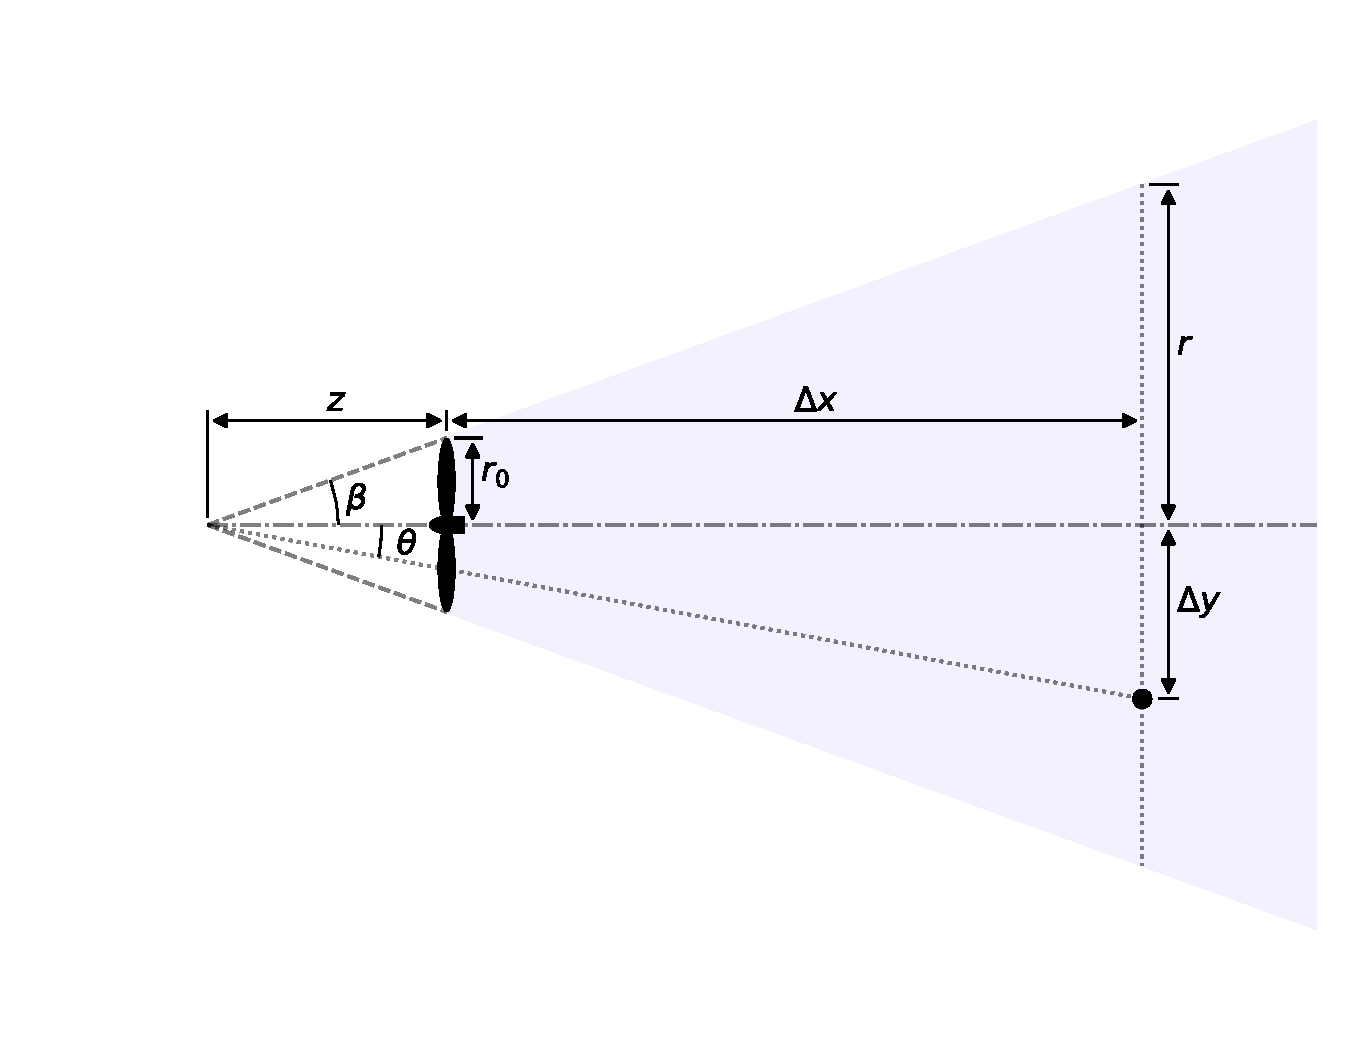
\includegraphics[width=\textwidth, trim={3cm 0cm 0cm 0cm}, clip]{wake_model_visualizations/jensen_diagram}
		\caption{Horizontal geometry of the Jensen cosine wake model. The wind is blowing to the right. The dashed line down the middle represents the center line of the wake. The large black dot represents any given point of interest.}
		\label{fig:JensenDiagrams}
	\end{subfigure}\hspace{1pc}
	\begin{subfigure}[t]{0.35\textwidth}
		\centering
		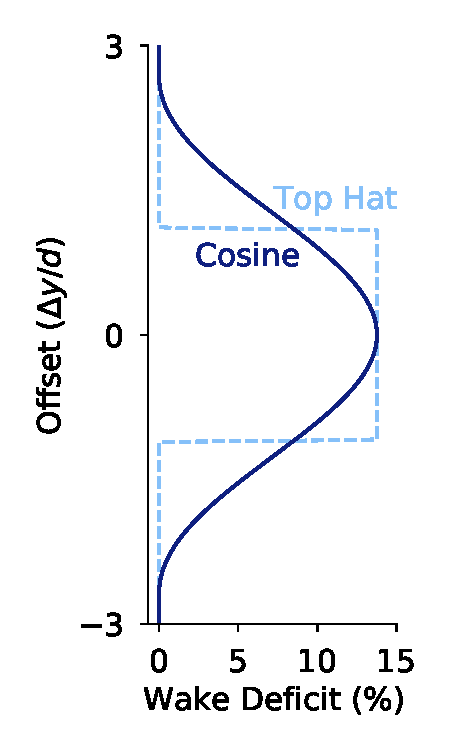
\includegraphics[width=0.6\textwidth, trim={1.05cm 0cm 1.05cm 0cm}]{wake_model_visualizations/jensen_profiles}
		\caption{Wake deficit profiles at 6 rotor diameters down wind for the Jensen top hat and Jensen cosine wake models.}
		\label{fig:JensenProfiles}
	\end{subfigure}
	\caption{The Jensen wake models \cite{jensen1983}.}
\end{figure}

\subsection{Turbine Model}
We based our turbines on the Vestas V-80 2MW wind turbine for all studies in this paper. The values of $C_P$ and $C_T$ were based on a linear interpolation of the power and thrust coefficient curves presented in \cite{niayifar2016} and shown in \cref{fig:cp,fig:ct}. The other turbine specifications are provide in \cref{tab:v80}. The $C_T$ curve was only used with the Bastankhah wake model. We used a constant axial induction value of 1/3 when using the Jensen cosine wake model.
%
\begin{figure}[h!]
	\centering
	\begin{minipage}[t]{0.48\textwidth}
		\centering
		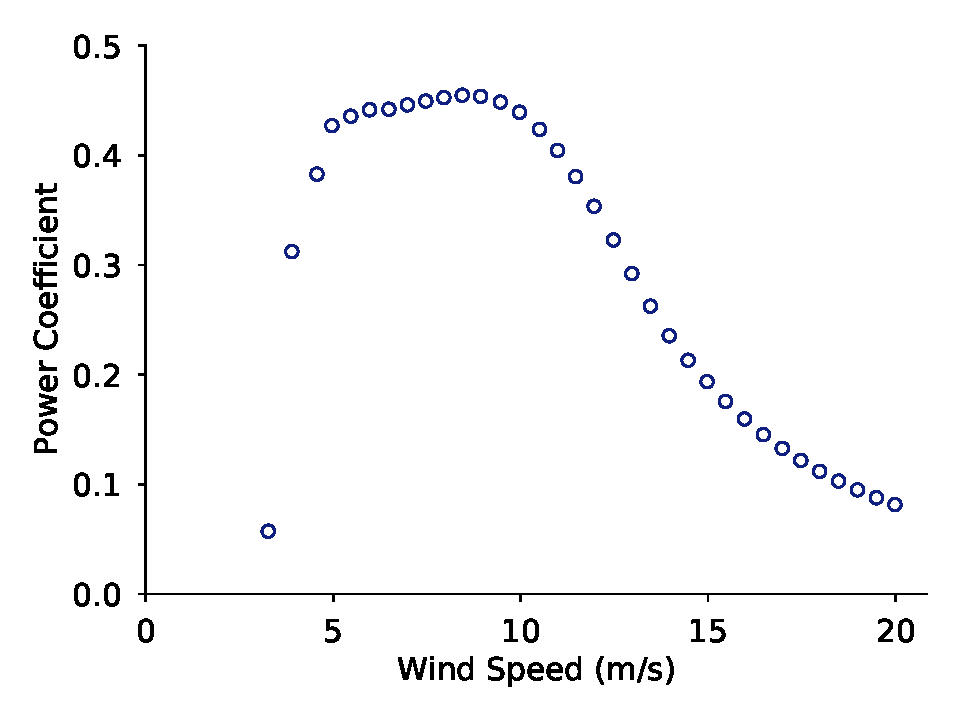
\includegraphics[width=\textwidth, trim={0cm 0cm 0cm 0cm}, clip]{inputs/cp_curve_v80}
		\caption{$C_P$ curve for the Vestas V80 2MW wind turbine \cite{niayifar2016} }
		\label{fig:cp}
	\end{minipage}\hspace{1pc}%
	\begin{minipage}[t]{0.48\textwidth}
		\centering
		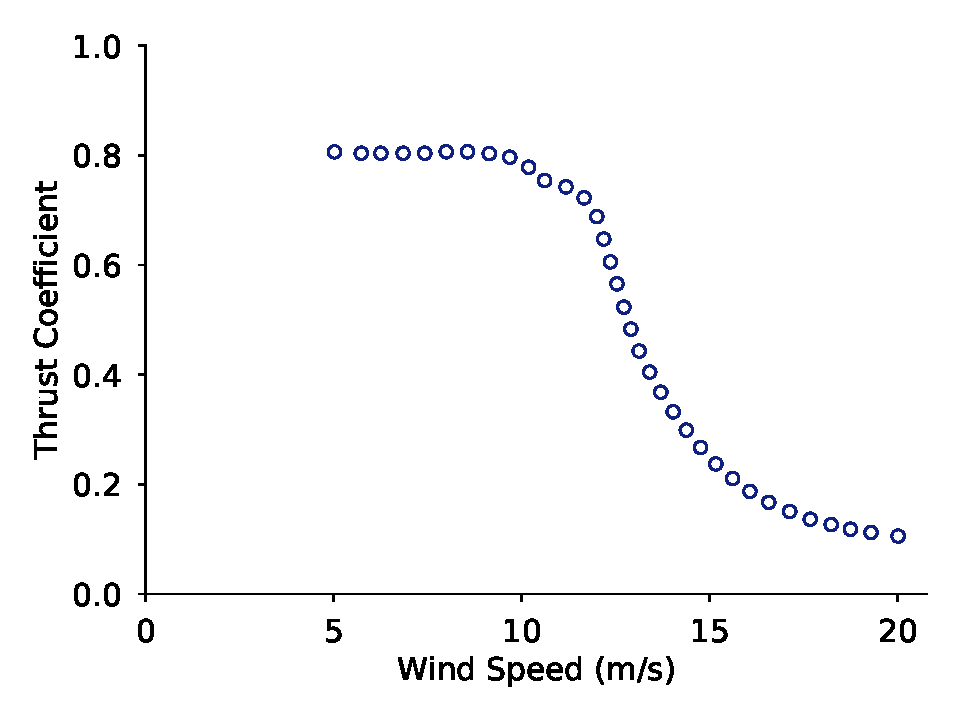
\includegraphics[width=\textwidth]{inputs/ct_curve_v80.pdf}
		\caption{$C_T$ curve for the Vestas V80 2MW wind turbine \cite{niayifar2016}}
		\label{fig:ct}
	\end{minipage} 
\end{figure}
%
\begin{table}[h!]
	\caption{Turbine Specifications}
	\label{tab:v80}
	\centering
	\begin{tabular}{l l}
		\br
		Rotor Diameter & 80.0 m\\
		Hub Height & 70.0 m \\
		Cut-in Speed & 4.0 m/s\\
		Cut-out Speed & 25.0 m/s \\
		Rated Speed & 16.0 m/s \\
		Rated Power & 2.0 MW \\
		Generator Efficiency & 0.944 \\
		\br
	\end{tabular}
\end{table}

\subsection{Other Models}
We combined the wake deficits using a linear combination method as discussed in \cite{niayifar2016} with the Bastankhah wake model, and a sum of squares method with the Jensen wake model as discussed in \cite{katic1986}. We used a reference height of 80 m for all wind speed measurements and adjusted to different heights with a power law and a wind shear exponent of 0.31 as shown in \cref{eq:shear}. 
%
\begin{equation} \label{eq:shear}
u = u_r\bigg[\frac{z}{z_r}\bigg]^\psi
\end{equation}
%
In \Cref{eq:shear}, $u_r$ is the reference wind speed, $z$ is the height of interest, $z_r$ is the height at which $u_r$ was measured, and $\psi$ is the shear exponent.

To save computation time, the inflow wind speed at each turbine was approximated using a single sample at the wind turbine hub location. Individual turbine inflow wind velocities, $U_i$, were solved consecutively from upstream to downstream for each wind state (direction and speed combination) for the Bastankhah wake model, but in no particular order for the Jensen cosine model. The power output of each turbine was then calculated based on \cref{eq:power}
%
\begin{equation}\label{eq:power}
P_i = \frac{1}{2}\rho A_{ri}C_P U_i^3
\end{equation}
%
where $\rho$ is the air density, $A_{r,i}$ is the rotor-swept area of turbine $i$, and $C_P$ is the power coefficient. We calculated annual energy production (AEP) as shown in \cref{eq:aep}.

\begin{equation} \label{eq:aep}
AEP = [24][365]\sum_{j=1}^{n_s} \sum_{i=1}^{n_t} p_j P_{ij}  
\end{equation}
%
 In \cref{eq:aep}, $n_s$ is the number of wind states (direction and speed combination), $p_j$ is the probability of a given wind state, $n_t$ is the number of wind turbines, and $P_{ij}$ is the power produced by turbine $i$ given wind state $j$.

To achieve an unbiased baseline for results comparisons, we calculated wake loss (energy lost due to wake effects) across all the optimization results as shown in \cref{eq:wake_loss}.
%
\begin{equation} \label{eq:wake_loss}
	L = 100 \bigg[ 1 - \frac{AEP_0}{AEP_t} \bigg]
\end{equation}
%
In \cref{eq:wake_loss}, $AEP_0$ represents the optimized AEP found from a given starting layout and $AEP_t$ is the theoretical maximum AEP calculated as shown in \cref{eq:aept}. 
%
\begin{equation} \label{eq:aept}
	AEP_t = [24][365]\sum_{j=1}^{n_s}p_j P_j
\end{equation}
%
In \cref{eq:aept}, $P_j$ is the power of a single un-waked wind turbine at wind state $j$ calculated using \cref{eq:power}. 

\section{Applying WEC to the  Wake Models} \label{sec:application}
In this section we apply WEC, step by step as discussed in \cref{sec:introwec}, to the Bastankhah wake model and the Jensen cosine wake model. To test the wake spreading approaches discussed, we implemented each of them in the Bastankhah  wake model. We then tested the most effective wake spreading approach with the Jensen cosine model.

\subsection{Applying WEC to the Bastankhah Wake Model}

\subsubsection{Bastankhah WEC Step (1)}
The first parenthetical term of \cref{eq:bpa} defines the magnitude of the velocity deficit. The exponential terms determine the wake spread. The wake spread and velocity deficit are coupled through $\sigma_y$ and $\sigma_z$. However, because the spread and magnitude are expressed in separate terms, it is possible to adjust one without impacting the other. 

\subsubsection{Bastankhah WEC Step (2) - WEC-D}
In the diameter spreading method (WEC-D), independent control of the wake diameter is obtained by introducing a factor, $\xi$, to $\sigma_y$ and $\sigma_z$ in the exponential terms of \cref{eq:bpa}, as shown in \cref{eq:bpa_relax}. The only change from \cref{eq:bpa} to \cref{eq:bpa_relax} is the addition of the WEC factor, $\xi$.
% \begin{equation}
% 	\frac{\Delta U}{U_{\infty}} = \Bigg(1-\sqrt{1-\frac{C_T}{8\sigma^2/d_0^2}}~\Bigg) \exp{\Bigg(-\frac{1}{2}\bigg(\frac{z-z_h}{\xi\sigma}\bigg)^2\Bigg)}\exp{\Bigg(-\frac{1}{2}\bigg(\frac{y-\delta}{\xi\sigma}\bigg)^2\Bigg)}
% 	 \label{eq:bpa_relax}
% \end{equation}
\begin{equation}
	\frac{\Delta \bar{u}}{\bar{u}_{\infty}} = \Bigg[1-\sqrt{1-\frac{C_T \cos{(\gamma)}}{8 \sigma_y \sigma_z/d^2}}~\Bigg] \exp{\bigg(-0.5\Big[\frac{y-\delta}{\xi \sigma_y}\Big]^2\bigg)}\exp{\bigg(-0.5\Big[\frac{z-z_h}{\xi \sigma_z}\Big]^2\bigg)}
	\label{eq:bpa_relax}
\end{equation}
Increasing $\xi$ widens the wakes without changing the wake center velocity deficit. Widened wakes mix and smooth out the local optima, as shown in \cref{fig:wec_bpa_wec_d}. 
%
%\begin{figure}[h!]
%	\centering
%	\begin{minipage}[t]{0.47\textwidth}
%		\centering
%		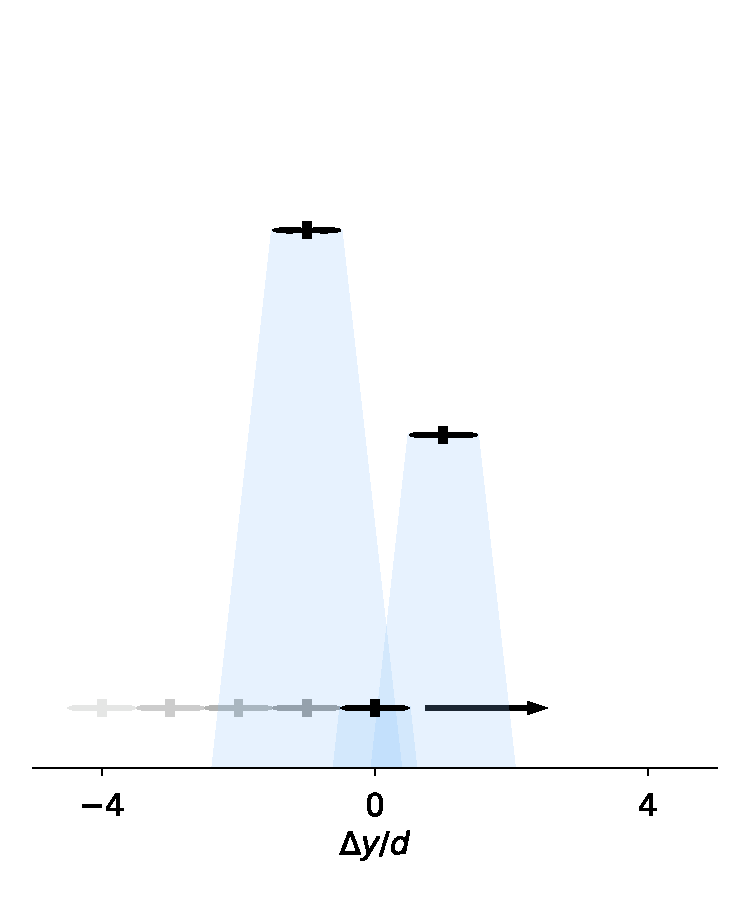
\includegraphics[width=\textwidth, trim={-2.0cm -0.0cm -2.0cm 3.5cm}, clip]{final_images/layouts/3turb-design-space}
%		\caption{Simple wind farm, seen from above, used to demonstrate the effects of the WEC factors, $\theta_\xi$ and $\xi$, on the wind farm layout design space (see \cref{fig:smoothing_bpa_wec_d}). Wind is from the top.}
%		\label{fig:smoothing_locations_bpa}
%	\end{minipage}\hspace{1pc}
%	\begin{minipage}[t]{0.47\textwidth}
%		\centering
%		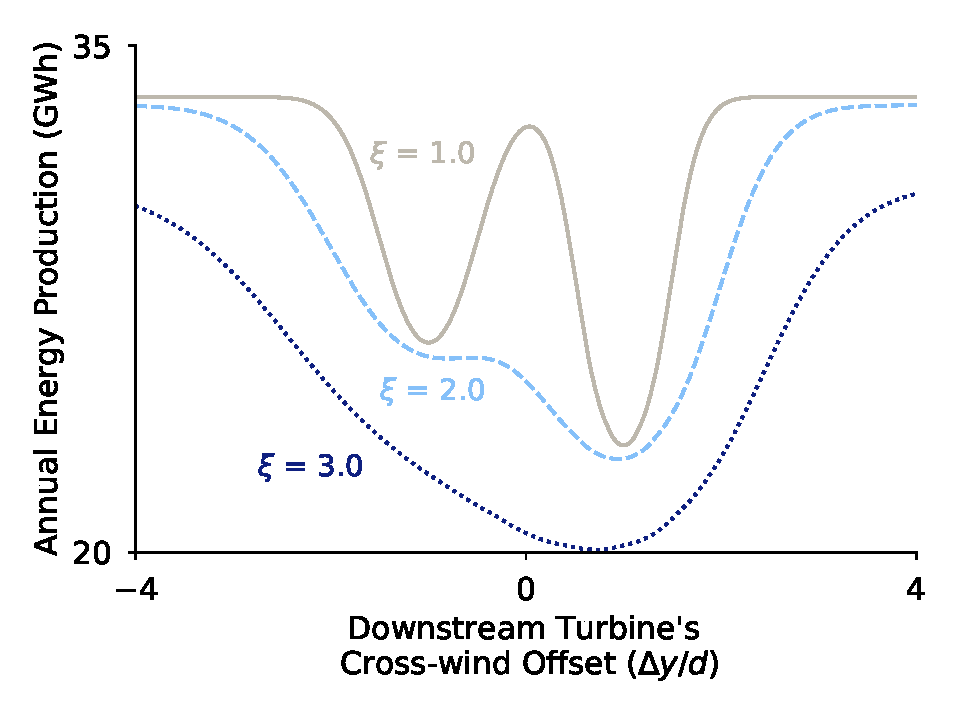
\includegraphics[width=\textwidth]{wake_model_visualizations/smoothing_bpa_wec_d}
%		\caption{The impact of the relaxation factor, $\xi$, for WEC-D on a simple wind farm layout design space with one movable turbine and one wind direction (see \cref{fig:smoothing_locations_bpa}) using the Bastankhah  wake model. The local optimum between the wakes disappears as the WEC factor increases.}
%		\label{fig:smoothing_bpa_wec_d}
%	\end{minipage} %\hspace{1pc}
%\end{figure}
\begin{figure}[h!]
	\centering
	\begin{subfigure}[t]{0.47\textwidth}
		\centering
		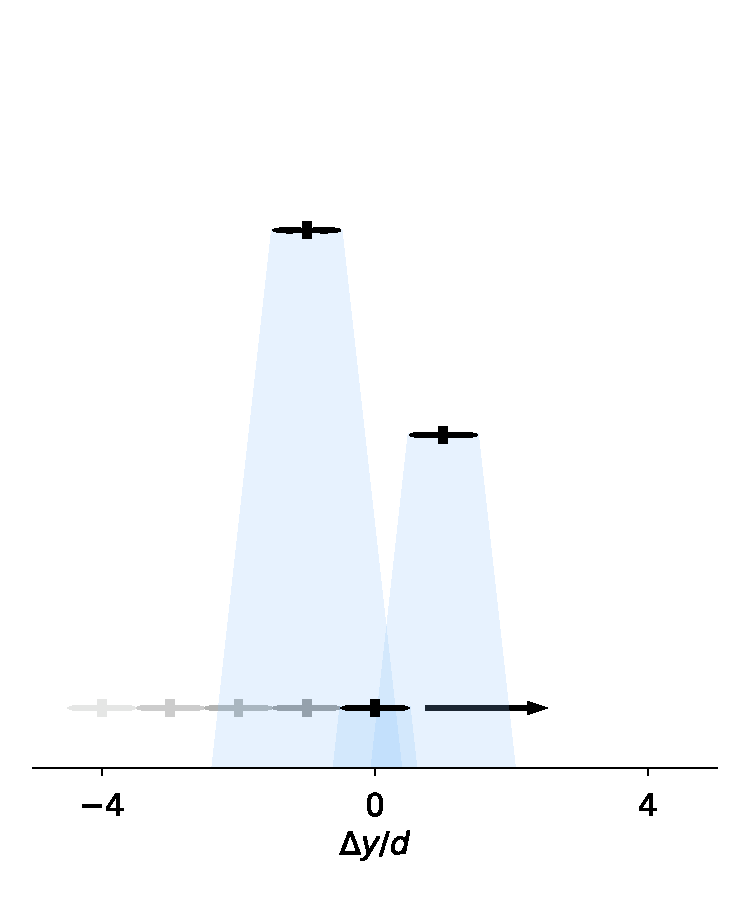
\includegraphics[width=\textwidth, trim={-2.0cm -0.0cm -2.0cm 3.5cm}, clip]{final_images/layouts/3turb-design-space}
	\caption{}
	\label{fig:smoothing_locations_bpa}
	\end{subfigure}\hspace{1pc}
	\begin{subfigure}[t]{0.47\textwidth}
		\centering
		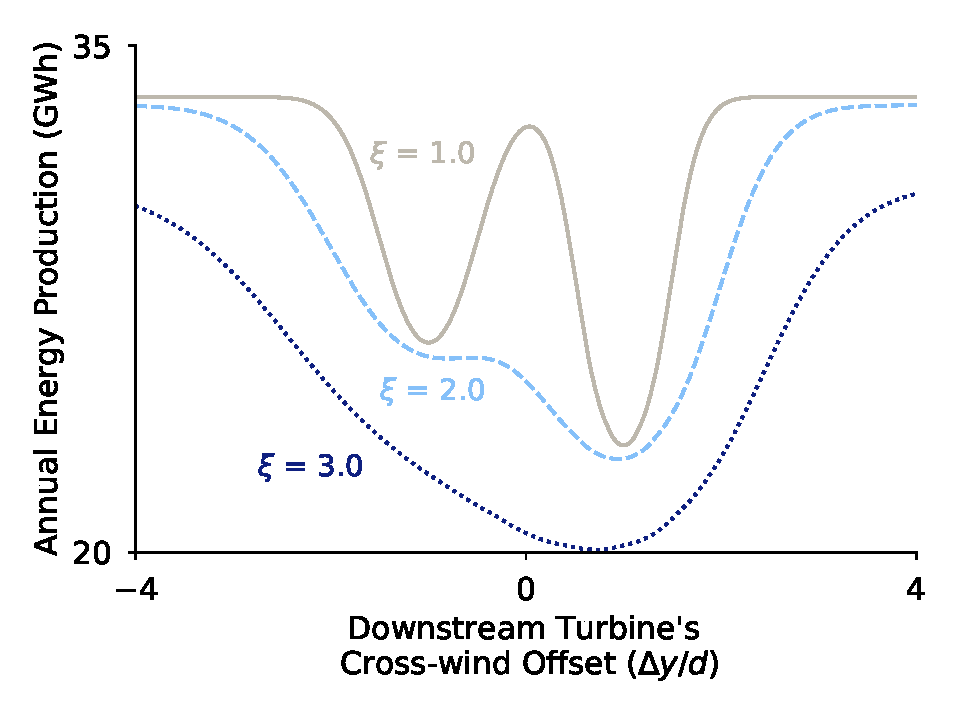
\includegraphics[width=\textwidth]{wake_model_visualizations/smoothing_bpa_wec_d}
		\caption{}
		\label{fig:smoothing_bpa_wec_d}
	\end{subfigure}
	\caption{The impact of the WEC factor, $\xi$, for WEC-D using the Bastankhah wake model. A simple wind farm with one movable turbine and one wind direction is shown from above in \cref{fig:smoothing_locations_bpa}. Wind is from the top. Increasing the WEC factor removes the local optima between the wakes of the two front turbines, as demonstrated in \cref{fig:smoothing_bpa_wec_d}.}
	\label{fig:wec_bpa_wec_d}
\end{figure}

\subsubsection{Bastankhah WEC Step (2) - WEC-A}
To gain direct control of the wake spreading angle, we arranged the equations in such a way that the user specifies the wake spreading angle, rather than using a multiple of the default angle. 

To gain direct control of the wake spreading angle, we calculate the wake spreading slope that would correspond to the desired spreading angle ($\theta_\xi$) and compare  it against the original spreading angle $k_{y_{\text{NEAR}}}$ (\cref{eq:kynear}) to obtain
%
\begin{equation}
	k_{y_{\xi}} = \max(\tan{(\theta_\xi)}, k_{y_{\text{NEAR}}})
\end{equation}
%
We then use $k_{y_{\xi}}$ to re-define the wake spread at the point of far wake onset, $\sigma_{y_{0A}}$, as shown in \cref{eq:sigmay0xi}.
%
\begin{equation}\label{eq:sigmay0xi}
	\sigma_{y_{0\text{A}}} = k_{y_{\xi}}x_0+\sigma_{yd}
\end{equation}
%
The definition for $\sigma_{y_{0\text{A}}}$ allows us to define the general form of the wake spread for all wake regions as shown in \cref{eq:sigmayxi}. 
%
\begin{equation}\label{eq:sigmayxi}
	\sigma_{y_{\text{A}}} =
	\begin{cases} k_y [x-x_0]+\sigma_{y_{0\text{A}}} & x >= x_0, k_y >= k_{y_{\xi}} \\
		k_{y_{\xi}} [x-x_0]+\sigma_{y_{0\text{A}}} & x >= x_0, k_y < k_{y_{\xi}} \\
		k_{y_{\xi}}x+\sigma_{yd} & x < x_0 \\
	\end{cases}
\end{equation}
%
We used the same process to obtain $\sigma_{z_{\text{A}}}$. 

Now that we have direct control of the wake spreading angle, for angles greater than the default angle, we can apply the results directly to the exponential terms of \cref{eq:bpa} to obtain a model that allows the user to specify a spreading angle without impacting the velocity deficit in the wake center as shown in \cref{eq:bpa_angle}. The only change from \cref{eq:bpa} to \cref{eq:bpa_angle} is replacing $\sigma_y$ and $\sigma_z$ in the exponential terms with $\sigma_{y_{\text{A}}}$ and $\sigma_{z_{\text{A}}}$ respectively.
\begin{equation}
	\frac{\Delta \bar{u}}{\bar{u}_{\infty}} = \Bigg[1-\sqrt{1-\frac{C_T \cos{(\gamma)}}{8 \sigma_y \sigma_z/d^2}}~\Bigg] \exp{\bigg(-0.5\Big[\frac{y-\delta}{\sigma_{y_{\text{A}}}}\Big]^2\bigg)}\exp{\bigg(-0.5\Big[\frac{z-z_h}{\sigma_{z_{\text{A}}}}\Big]^2\bigg)}
	\label{eq:bpa_angle}
\end{equation}
%
For WEC-A, The impact of $\theta_\xi$ is much more pronounced for turbines that are further upstream due to the increased wake growth rate, but are otherwise similar to the effects shown for WEC-D in \cref{fig:smoothing_bpa_wec_d}.

\subsubsection{Bastankhah WEC Step (2) - WEC-H}

The third approach, WEC-H, is a hybrid of WEC-D and WEC-A. The wake diameter is multiplied in the far wake, but the near wake expands linearly until the point where the wake diameter multiplier is applied as shown in \cref{eq:sigywech}.
%
\begin{align}\label{eq:sigywech}
	\sigma_{y_H} = &
	\begin{cases}
		\xi \sigma_y & x > x_0 \\
		\xi \big[\frac{x}{x_0}[\sigma_{y_0} - \sigma_{y_d}] + \sigma_{y_d} \big]& x \le x_0 \\
	\end{cases}
\end{align}
%
Where $\sigma_{y_0}$ is the original wake spread at $x_0$, and $\sigma_{y_H}$ is the horizontal wake standard deviation to be used in the exponential terms of the Bastankhah model as shown in \cref{eq:wechapplied}. A similar approach can be used to find $\sigma_{z_H}$. The Bastankhah model with WEC-H applied is shown in \cref{eq:sigywech}. The only change from \cref{eq:bpa} to \cref{eq:wechapplied} is replacing $\sigma_y$ and $\sigma_z$ in the exponential terms with $\sigma_{y_{H}}$ and $\sigma_{z_{H}}$ respectively.

\begin{equation}
	\frac{\Delta \bar{u}}{\bar{u}_{\infty}} = \Bigg[]1-\sqrt{1-\frac{C_T \cos{(\gamma)}}{8 \sigma_y \sigma_z/d^2}}~\Bigg] \exp{\bigg(-0.5\Big[\frac{y-\delta}{ \sigma_{y_H}}\Big]^2\bigg)}\exp{\bigg(-0.5\Big[\frac{z-z_h}{ \sigma_{z_H}}\Big]^2\bigg)}
	\label{eq:wechapplied}
\end{equation}

Note that the $\sigma_{y_H}$ term is only applied to the wake width terms and the original model values are used in calculating the magnitude of the center-line wake deficit. As in WEC-A and WEC-D, increasing the value of the WEC factor, $\xi$, allows us to widen the wake without changing the magnitude of the velocity deficit in the center of the wake. As the wakes widen, they mix and smooth out the local optima. The effects are similar to those shown for WEC-D in \cref{fig:smoothing_bpa_wec_d}.

\subsubsection{Bastankhah WEC Step (3)}
To gain the benefits of WEC without losing the accuracy of the wake model, the optimization must be run multiple times, in a continuation approach, with values of $\xi$ or $\theta_\xi$ decreasing to 1 or 0 respectively. The results from optimizing with each value of $\xi$ or $\theta_\xi$ can then be used to warm start the next optimization. In this way, the gradient-based optimization can intelligently explore the design space and then refine the model to find a final, more accurate, result. The iterative optimizations are generally fairly fast due to starting from the previous optimized solution. In \cref{sec:tuning}, we will show how we determined which WEC method to use and the corresponding values of $\xi$ or $\theta_\xi$ to use in practice.

\subsection{Applying WEC to the Jensen Cosine Wake Model}
In this section we apply WEC-D to the Jensen cosine wake model. A diagram displaying the Jensen cosine wake model from an overhead perspective is shown in \cref{fig:JensenDiagrams}. The diagram will give context to the variables and parameters discussed in this section.

\subsubsection{Jensen Cosine WEC Step (1)} 
%Identify where the magnitude and spread of the wake are within the Jensen Cosine equation.

The cosine factor, $f_\theta$, in \cref{eq:JensenVelocityDeficit} controls the wake spread for the Jensen cosine wake model. By breaking down the cosine factor into its constituent parameters, it is possible to adjust the wake spread without impacting the velocity deficit in the center of the wake.

As can be seen in \cref{eq:JensenCosineAdjustment}, $f_\theta$ is a function of $\theta$, which represents the angle between the wake's center line and the downwind turbine's location as measured from the wake vertex (a distance $z$ along the wake center line upstream of the wind turbine). This angle $\theta$ can be determined using \cref{eq:Theta}.

% Equation for calculating theta, the angle between the wake's vertex and the point of interest
\begin{equation}
	\theta = \arctan\Big( \frac{\Delta y}{\Delta x + z} \Big)
	\label{eq:Theta}
\end{equation}

In \cref{eq:Theta}, $\Delta x$ and $\Delta y$ represent the downwind and crosswind spacing, respectively, between the upwind turbine and the downwind location of interest. The variable $z$ represents the distance between the wake's vertex and the upwind turbine. By adjusting the value of $z$, we are able to increase or decrease the wake's spread. An expression for $z$ based on the initial wake diameter can be found below in \cref{eq:vertexdistance}.

\begin{equation}
	z = \frac{r_0}{\tan(\beta)}
	\label{eq:vertexdistance}
\end{equation} 


\subsubsection{Jensen Cosine WEC Step (2)}
We can directly adjust the wake spread without impacting the magnitude of the deficit in the center of the wake by applying a relaxation factor, $\xi$, to the rotor radius, $r_0$, in \cref{eq:vertexdistance}, as seen below in \cref{eq:WECvertexcistance}.

\begin{equation}
	z = \frac{\xi r_0}{\tan(\beta)}
	\label{eq:WECvertexcistance}
\end{equation}

Through a series of substitutions, this new vertex distance, \cref{eq:WECvertexcistance}, may be combined with the Jensen cosine wake model to obtain \cref{eq:JensenVelocityDeficitCombined}.

% Insert equation: final equation displaying the direct relationship between the velocity deficit and the relaxation factor, xi.
\begin{equation}
	\frac{\Delta \bar{u}}{\bar{u}_\infty} = 1 - a \bigg[\frac{r_0}{r_0 + \alpha x} \bigg]^2 \Bigg[1 + \cos{\Bigg(\frac{\pi}{\beta} \arctan{\Bigg(\frac{\Delta y}{\Delta x + \frac{\xi r_0}{\tan(\beta)}}} \Bigg) \Bigg)} \Bigg]
	\label{eq:JensenVelocityDeficitCombined}
\end{equation}

Because we have inserted the relaxation factor, $\xi$, into \cref{eq:JensenVelocityDeficitCombined}, we may adjust the wake spread without changing the velocity deficit in the center of the wake. Note that this is true because when $\Delta y = 0$, the term inside the inverse tangent in \cref{eq:JensenVelocityDeficitCombined} goes to zero, regardless of the value of $\xi$. Because this is the only place where the relaxation factor is found in \cref{eq:JensenVelocityDeficitCombined}, this means that the velocity deficit will be constant with respect to $\xi$ at the wake center. This behavior is shown in \cref{fig:wec_jensen_wec_d}, which also shows that local optima can be smoothed out through WEC for the Jensen cosine model.

% Figure describing setup for aep vs crosswind position tests for Jensen
%\begin{figure}[ht]
%	\centering
%	\begin{minipage}[t]{0.43\textwidth}
%		\centering
%		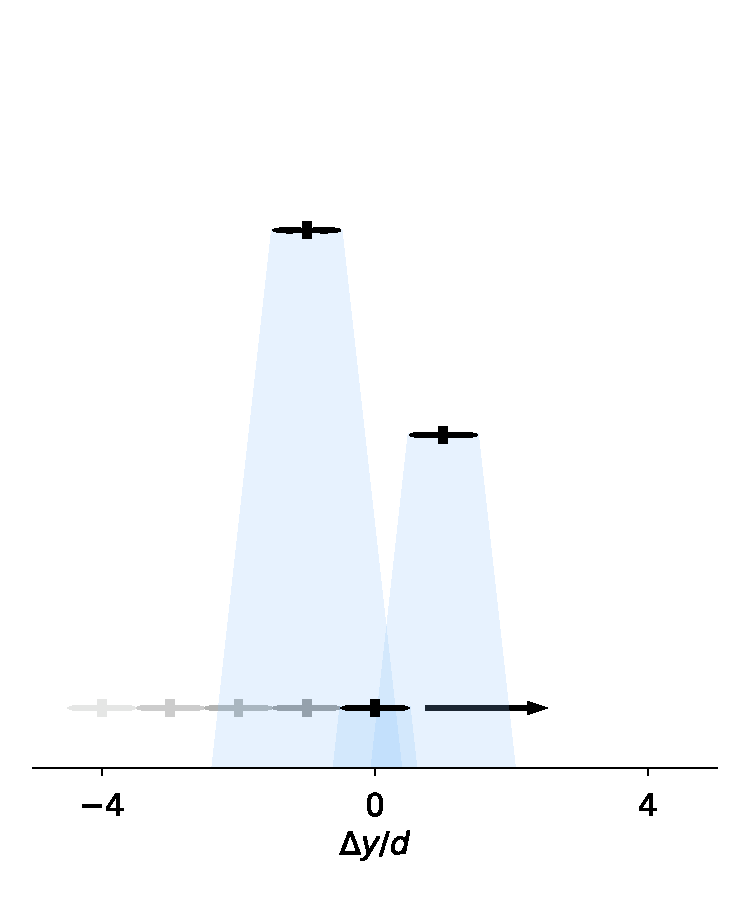
\includegraphics[width=\textwidth, trim={-0.5cm -0.5cm -0.5cm 3.25cm}, clip]{final_images/layouts/3turb-design-space}
%		\caption{Simple wind farm, seen from above, used to demonstrate the effects of the WEC factor $\xi$, on the wind farm layout design space (see \cref{fig:smoothing_jensen_wec_d}). Wind is from the top.}
%		\label{fig:smoothing_locations_jensen}
%	\end{minipage}\hspace{1pc}
%	% Figure displaying results from aep vs crosswind position tests for Jensen
%	\begin{minipage}[t]{0.52\textwidth}
%		\centering
%		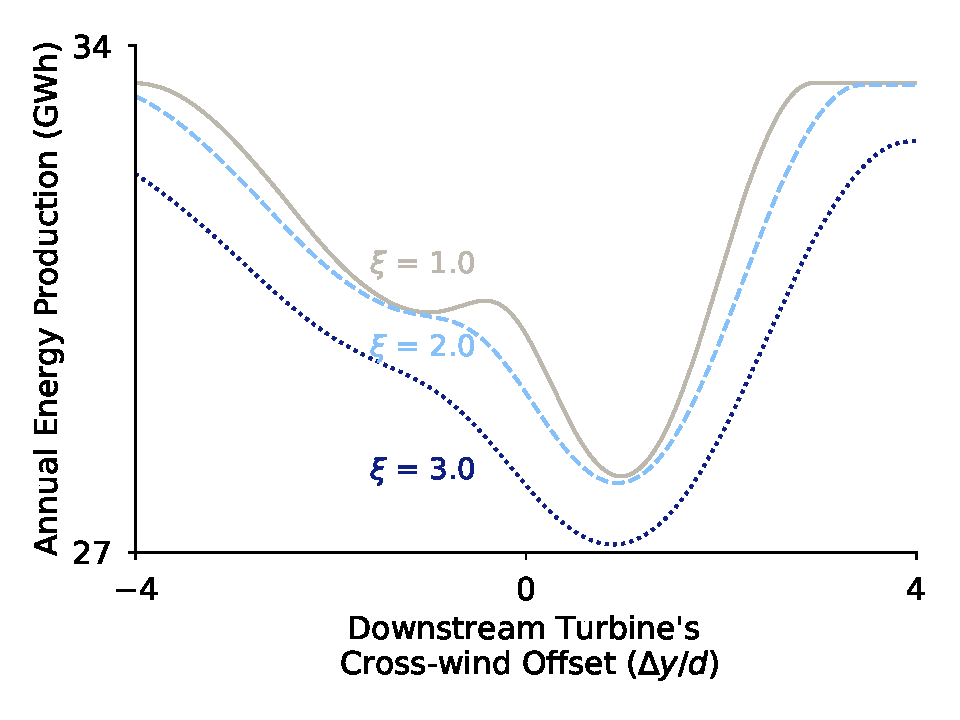
\includegraphics[width=\textwidth]{wake_model_visualizations/smoothing_jensen_wec_d}
%		\caption{The impact of changing the WEC factor, $\xi$, for WEC on a simple wind farm layout design space with one movable turbine and one wind direction (see \cref{fig:smoothing_locations_jensen}) using the Jensen cosine wake model. The local optimum between the wakes disappears as the WEC factor increases.}
%		\label{fig:smoothing_jensen_wec_d}
%	\end{minipage}
%\end{figure}

\begin{figure}[h!]
	\centering
	\begin{subfigure}[t]{0.47\textwidth}
		\centering
		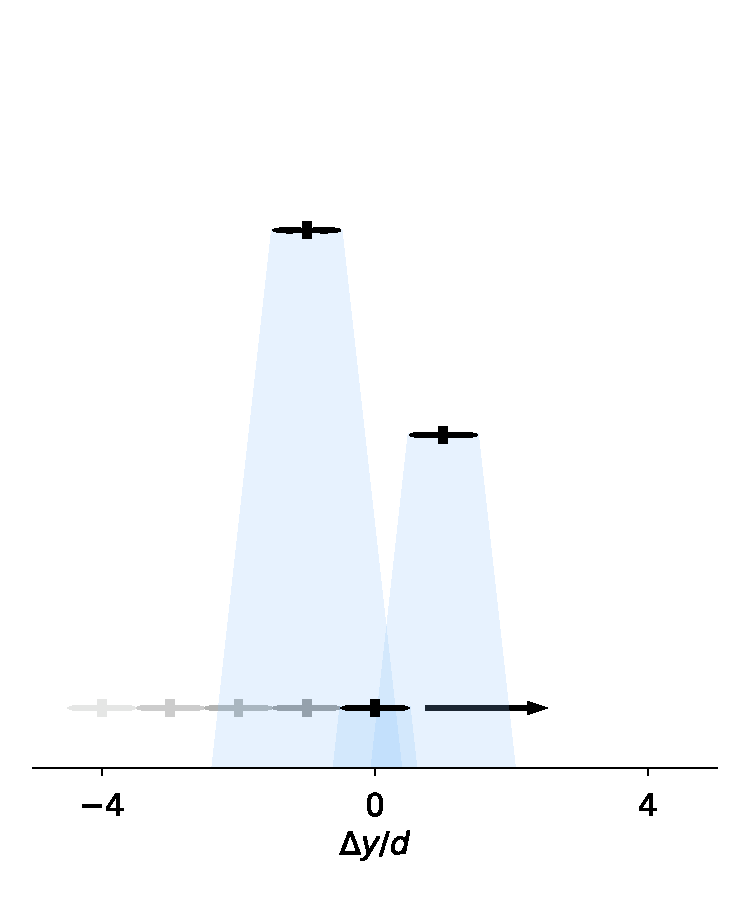
\includegraphics[width=\textwidth, trim={-2.0cm -0.0cm -2.0cm 3.5cm}, clip]{final_images/layouts/3turb-design-space}
		\caption{}
	\label{fig:smoothing_locations_jensen}
	\end{subfigure}\hspace{1pc}
	\begin{subfigure}[t]{0.47\textwidth}
		\centering
		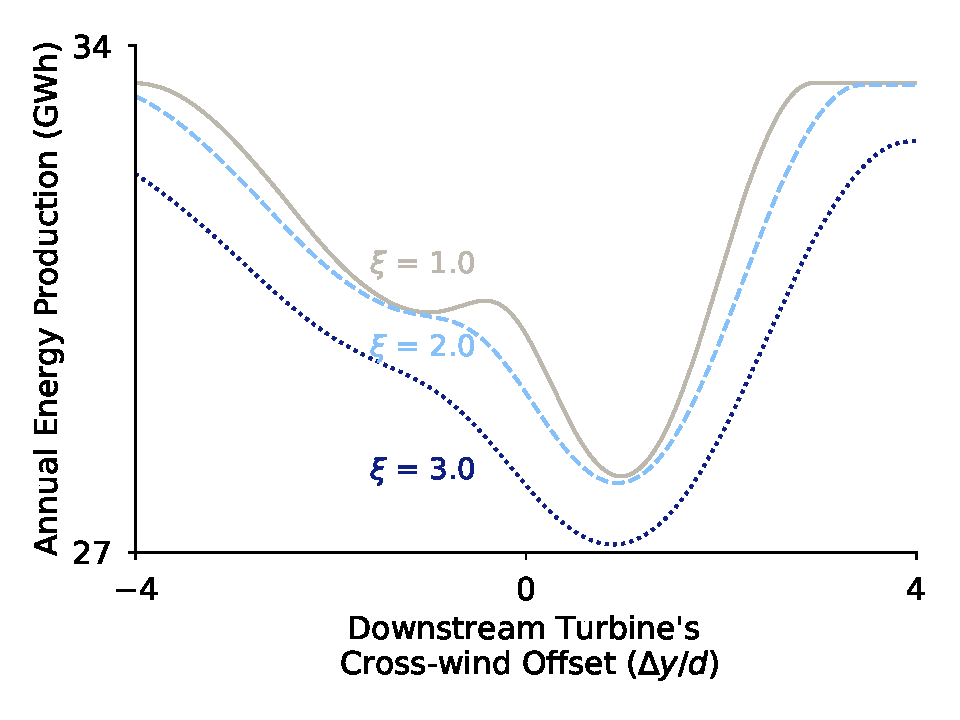
\includegraphics[width=\textwidth]{wake_model_visualizations/smoothing_jensen_wec_d}
		\caption{}
		\label{fig:smoothing_jensen_wec_d}
	\end{subfigure}
	\caption{The impact of the WEC factor, $\xi$, for WEC-D using the Jensen cosine wake model. A simple wind farm with one movable turbine and one wind direction is shown from above in \cref{fig:smoothing_locations_jensen}. Wind is from the top. Increasing the WEC factor removes the local optima between the wakes of the two front turbines, as demonstrated in \cref{fig:smoothing_jensen_wec_d}.}
	\label{fig:wec_jensen_wec_d}
\end{figure}

\subsubsection{Jensen Cosine WEC Step (3)}

The final step of the WEC method is the same for all models, with the exception that different WEC factors and number of WEC steps may be optimal for different wake models.

%\subsection{Testing WEC with ALPSO}
%
%Beside knowing if WEC works with different wake models, it is also of interest to know if WEC can improve the results of gradient-free algorithm. To test this we ran the same case shown in \cref{fig:round_case,fig:nantucket12dirs} using ALPSO with and without WEC. The results of this test are shown in \cref{
%
%\begin{figure}[h!]  
%	\centering
%	\begin{minipage}[t]{18pc}    
%		\centering
%		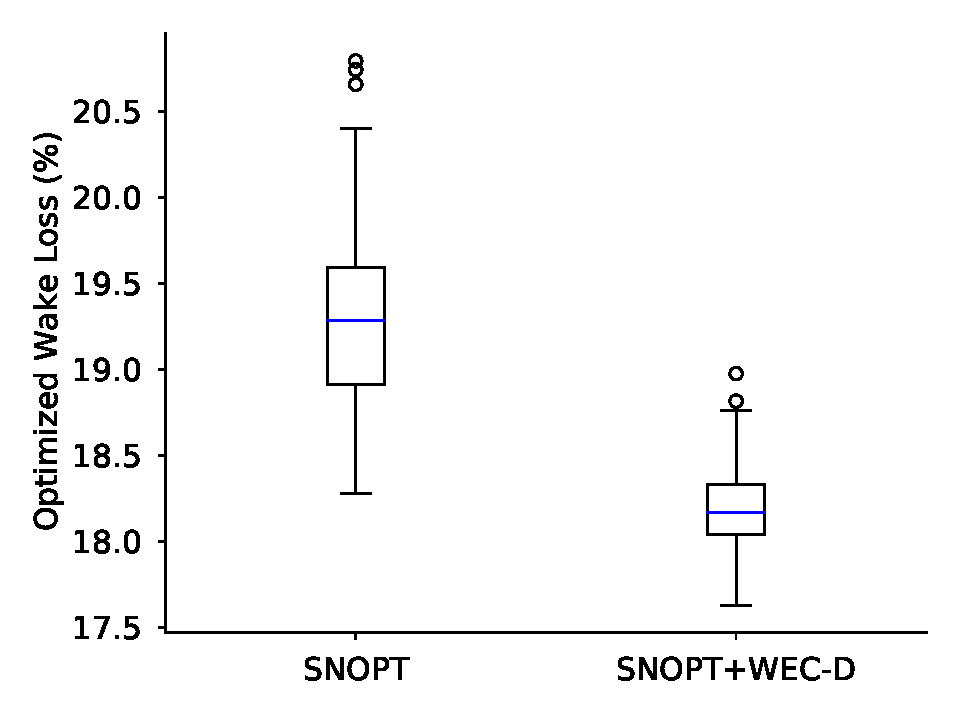
\includegraphics[width=\textwidth, trim={0cm 0cm 0cm 0cm}]{final_images/results/38turbs_results_jensen_percent_wake_loss.pdf}
%		\caption{Wake loss percentage for 200 optimizations using the Jensen model with and without WEC. These optimizations were performed on the 38 turbine wind farm and 12 direction wind rose shown in \cref{fig:method_study_layout,fig:nantucket12dirs}.}
%		\label{fig:jensen-38-wake-loss}
%	\end{minipage}\hspace{1pc}
%	\begin{minipage}[t]{18pc}    
%		\centering
%		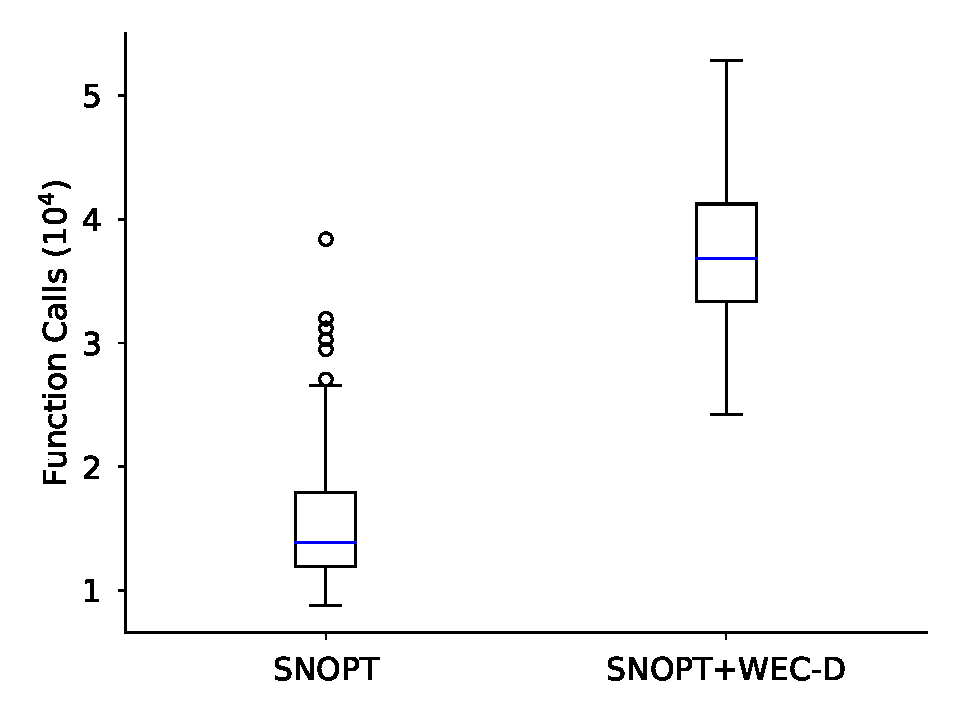
\includegraphics[width=\textwidth, trim={0cm 0cm 0cm 0cm}]{final_images/results/38turbs_results_jensen_fcalls.pdf}
%		\caption{Function calls for 200 optimizations using the Jensen model with and without WEC. These optimizations were performed on the 38 turbine wind farm and 12 direction wind rose shown in \cref{fig:method_study_layout,fig:nantucket12dirs}.}
%		\label{fig:jensen-38-wake-fcalls}
%	\end{minipage}
%\end{figure}

%\subsection{Applying WEC to the FLORIS Wake Model}
%In this section we apply WEC, step by step, as presented in \cref{sec:dsrop} to the FLORIS wake model.  
%
%%\todo{need to get better figure. remember to update caption once new figure inserted.}
%%\begin{figure}[h]
%%    \centering
%%    \includegraphics[width=0.3\linewidth]{FLORISDiagram1}
%%    \caption{Diagram displaying the three wake zones in the FLORIS turbine wake model. A higher quality diagram would have been constructed if there had been sufficient time. The black outer lines represent the outermost wake zone (mixing zone) which expands from the wind turbine as the air travels downstream. The blue lines represent the middle wake zone (far zone) which retains nearly the same width with distance from the turbine. Finally, the green lines represent the innermost wake zone (near wake) which converges to a point some distance from the turbine. The velocity deficit associated with each wake zone increases from the outermost wake zone to the innermost wake zone.}
%%    \label{fig:FLORISDiagram}
%%\end{figure}
%
%\subsubsection{FLORIS WEC Step (1)}
%%\textbf{Identify where the magnitude and spread of the wake are within the FLORISSE equation.}
%
%We began by determining where in the FLORIS wake model to apply the relaxation factor. Similar to the Jensen cosine wake model, we decided to apply the relaxation factor to the original wake diameter in the FLORIS wake model. Because the increased wakes would result in larger wake overlaps, we decided that our implementation of WEC would need to occur before any area overlap calculations took place. Based on Figure 3 of Gebraad et. al's paper \cite{gebraad2014}, we decided that the most intuitive option would be to implement the relaxation factor in the wake diameter equation (\cref{eq:FLORISWakeWidth}).
%
%\begin{equation}
%    D_{w,i,q} = D_i + 2k_em_{e,q}(x - X_i)
%    \label{eq:FLORISWakeWidth}
%\end{equation}
%
%In \cref{eq:FLORISWakeWidth}, $D_{w,i,q}$ represents the diameter of the wake for the turbine of index $i$ within the wake-zone $q$, $D_i$ represents the rotor-diameter of turbine $i$, $k_e$ and $m_{e,q}$ represent wake expansion coefficients, $x$ represents the distance downwind from the wake-generating turbine to turbine $i$, and $X_i$ represents the x-coordinate of turbine $i$. In this equation, $k_e$ and $m_{e,q}$ determine the rate of expansion while $D_i$ represents an initial wake width.
%
%\subsubsection{FLORIS WEC Step (2)}
%%\textbf{Apply relaxation factor to the FLORIS equation. Show the aep vs crosswind position plot to demonstrate the velocity deficit is unchanged in the center of the wake and that the wakes are capable of being spread out. Briefly describe this plot and how the wec factor affects it.}
%
%If we applied the relaxation factor to $k_e$ or $m_{e,q}$ in \cref{eq:FLORISWakeWidth}, the rate of wake expansion would be affected, which violates the conditions for WEC described at the start of the Methods section. On the other hand, applying the relaxation factor to $D_i$ would expand the wake without affecting the rate of wake expansion. Therefore, we decided to apply the relaxation factor to $D_i$ in \cref{eq:FLORISWakeWidth} to obtain \cref{eq:FLORISWECWakeWidth}.
%
%\begin{equation}
%    D_{w,i,q}' = D_i' + 2k_em_{e,q}(x - X_i)
%    \label{eq:FLORISWECWakeWidth}
%\end{equation}
%
%Where $D_{w,i,q}'$ represents the adjusted wake width from applying WEC and $D_i'$ represents the adjusted initial wake diameter from applying WEC. We applied a relaxation factor to all wake zones within the FLORIS wake model. The resulting equations controlling the wake diameters for various wake zones in the FLORIS model are displayed below in \cref{eq:FLORISWECWakeDiameterPiecewise}. In this equation, $q$ represents the wake zone being used (i.e., $q = 1$ for the innermost wake zone, $q = 2$ for the middle wake zone, and $q = 3$ for the outermost wake zone).
%
%%\begin{equation}
%%    D_i' = \xi D_i
%%    \label{eq:FLORISWECWakeDiameter}
%%\end{equation}
%
%% Initial results from applying the above equations prompted us to adjust our methods. First, we decided to implement a cosine factor to smooth the results, as done by Thomas and Ning in \cite{Thomas2017}. Second, we noticed that the preliminary results from FLORIS indicated that the velocity deficit in the wake's center was not constant for all values of $\xi$. We determined that the cause of this error was the increase in wake width of the innermost wake-zone. By increasing this wake diameter, we were allowing the innermost wake-zone to propagate much farther downwind than it would without a relaxation factor. Thus, turbines near the center of the wake would experience the effects of the innermost wake-zone for high values of $\xi$ but not for lower values of $\xi$. This caused the velocity deficit in the center of the wake to differ with $\xi$.
%
%% Originally, we resolved this issue by only applying the WEC relaxation factor to the middle and outermost wake zones. By doing so, we kept the innermost zone from propagating too far downstream and thereby ensured that the velocity deficit at the wake-center would be the same for all $\xi$. After more testing, however, we determined that failing to apply the relaxation factor to the innermost wake zone actually promoted the creation of a local optimum between two upwind turbines, which defeats WEC's purpose in smoothing out local optima. While the velocity deficit in the center of the wake is not preserved as well when applying WEC to the innermost wake zone, FLORIS performs better with WEC as a result of this change.
%
%\begin{equation}
%	D_{w, i, q}' = \xi D_i + 2k_em_{e, q} (x - X_i), q = 1, 2, 3
%	\label{eq:FLORISWECWakeDiameterPiecewise}
%\end{equation}
%
%When we applied \cref{eq:FLORISWECWakeDiameterPiecewise} to the FLORIS wake model, we tested how well WEC performed by traversing a turbine through the wakes of two fixed upwind wind turbines, similar to what was done with the Jensen cosine wake model in \cref{fig:smoothing_locations_Jensen,fig:JensenLocalOptSmoothed}. Our results are displayed in \cref{fig:smoothing_locations_FLORIS,fig:FLORISLocalOptSmoothed} below. We expected that the local optimum would be progressively smoothed out as the relaxation factor increased, similar to what is seen in \cref{fig:JensenLocalOptSmoothed}; however, as seen in \cref{fig:smoothing_locations_FLORIS,fig:FLORISLocalOptSmoothed}, WEC enabled the FLORIS model to smooth out the local optimum with only a small increase in the relaxation factor.
%
%% Figure describing setup for aep vs crosswind position tests for FLORIS
%\begin{figure}[ht]
%	\centering
%	\begin{minipage}[t]{0.43\textwidth}
%		\centering
%		\includegraphics[width=\textwidth, trim={2cm 0cm 2cm 0cm}, clip]{smoothing_locations}
%		\caption{Simple design space used to demonstrate the effects of the relaxation factor, $\xi$, on the wind farm layout design space (see \cref{fig:FLORISLocalOptSmoothed}).}
%		\label{fig:smoothing_locations_FLORIS}
%	\end{minipage}\hspace{1pc}
%% Figure displaying results from aep vs crosswind position tests for FLORIS
%	\begin{minipage}[t]{0.52\textwidth}
%		\centering
%		\includegraphics[width=\textwidth]{FLORISWECMultipleTurbinesAEP}
%		\caption{AEP plotted against crosswind position of the turbine seen in \cref{fig:smoothing_locations_FLORIS}. Drops in AEP occur where wakes are present. Note the local optimum between the two wakes that is smoothed out as the WEC factor increases.}
%		\label{fig:FLORISLocalOptSmoothed}
%	\end{minipage}
%\end{figure}
%
%\subsubsection{FLORIS WEC Step (3)}
%%\textbf{Describe how the optimization would actually use WEC (e.g., multiple wec factors decreasing from some value to 1, at which point the model is normal again. Warm start new optimizations with previous optimization's results). Report which values for wec factor were used.}
%
%The optimization for the FLORIS model with WEC is simple in concept. A reasonably large relaxation factor is chosen for the first optimization, which results in an optimized wind farm layout where all local optima have been smoothed out. A new, lower relaxation factor is chosen, and the results from the previous optimization are used as a warm start for the new optimization. This process repeats until the relaxation factor is equal to one, at which point the optimization being solved is identical to optimizing the original FLORIS model without WEC. In this way, WEC allows the optimization to escape local optima in the first few optimizations, but the FLORIS model becomes more accurate as the relaxation factor is decreased closer to one. Through trial and error, we decided to use the following relaxation factors: $\xi = [3, 2.75, 2.5, 2.25, 2, 1.75, 1.5, 1.25, 1]$. The selection of relaxation factors should be the topic of future research.

\section{Case Studies}\label{sec:casestudies}
To demonstrate the effectiveness of WEC on a range of problems, we present three wind farm optimization case studies. For each case, we used the Vestas V-80 2MW wind turbine. The cases were chosen to represent a range in size, complexity, and difficulty of the optimization problem.

We created 199 pseudo-random starting wind farm layouts and one planned layout for each case for a total of 200. Each of the starting layouts had all the turbines inside the wind farm boundary constraint and did not have any turbines spaced less than one rotor diameter apart.

\subsection{Case 1: 16 Turbines and 20 Wind Directions}
Case 1 was carefully selected to provide a meaningful problem that would be tractable for nearly any optimization method. We defined a wind farm with 16 wind turbines and a square boundary with enough space for four rows and columns of wind turbines with a five rotor diameter spacing between rows and columns (see \cref{fig:layout1}). We used a simple wind rose composed of a double Gaussian distribution binned into 20 directions and a constant wind speed of 10 m/s in all directions (see \cref{fig:directional}).
\begin{figure}[h!]
\centering
\begin{minipage}[t]{18pc}
\centering
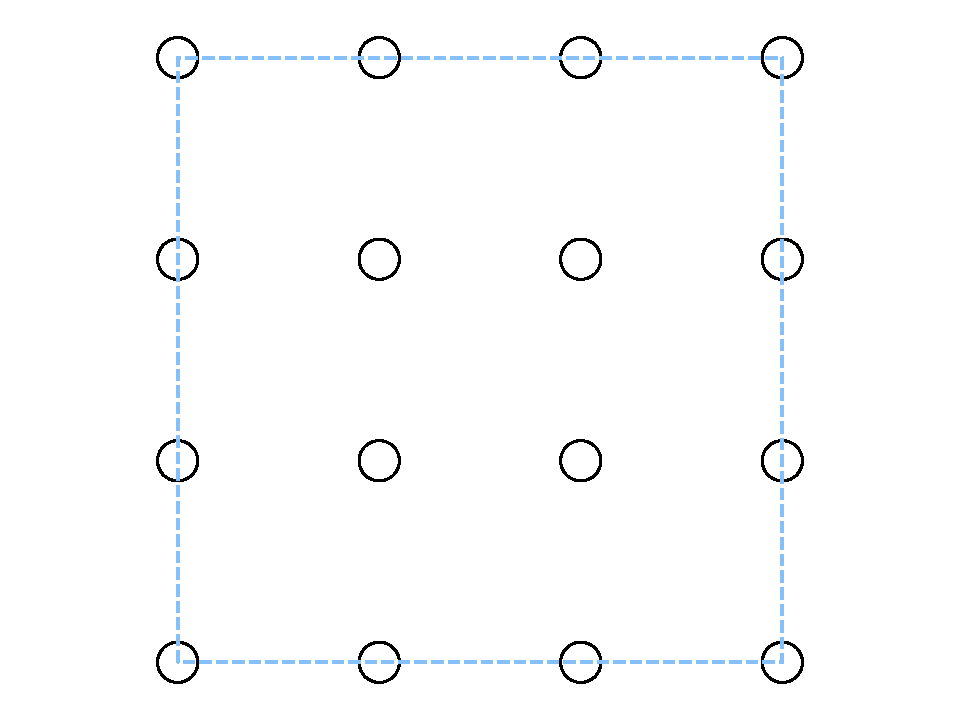
\includegraphics[width=1.\textwidth, trim={1.5cm, 0cm, 1.5cm, 0cm}, clip]{final_images/layouts/16_turb_start.pdf}
\caption{Baseline wind farm layout for case 1. The circles marking turbine locations are to scale, with diameters equal to the rotor diameter.}
\label{fig:layout1}
\end{minipage}\hspace{1pc}%
\begin{minipage}[t]{18pc}
\centering
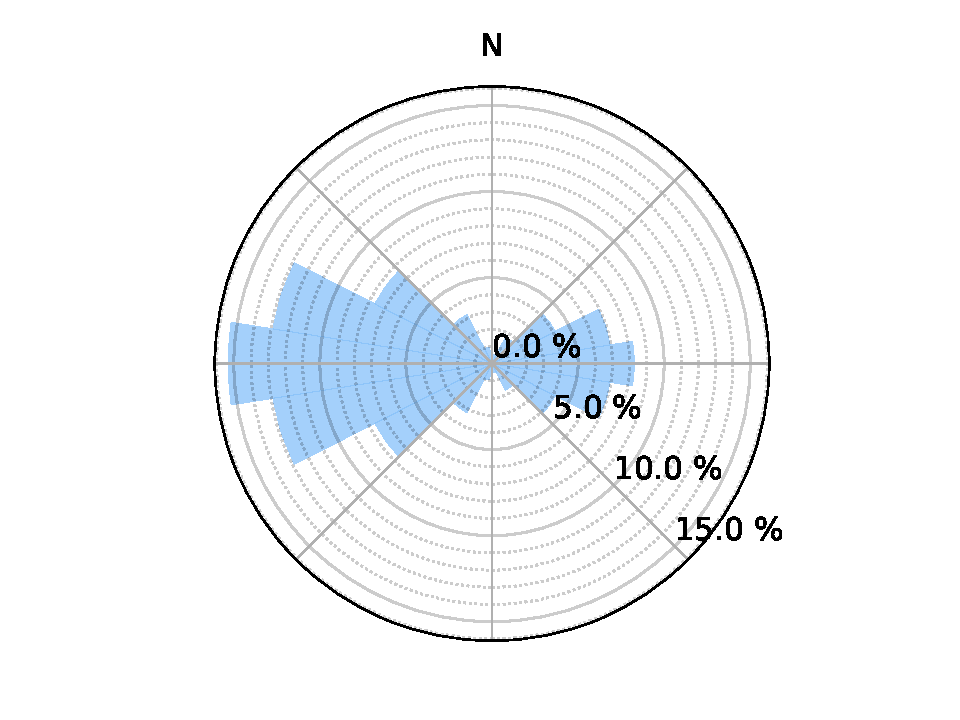
\includegraphics[width=\textwidth, trim={2.0cm 0cm 2.0cm 0cm}, clip]{final_images/windroses/freqwindrose_20_dir.pdf}
\caption{Direction probability wind rose for case 1. This wind rose is composed of a double Gaussian distribution binned into 20 directions.}
\label{fig:directional}
\end{minipage} 
\end{figure}
%

For case 1, the optimization problem was formulated as shown in \cref{eqn:opt1}
%
\begin{equation}
	\label{eqn:opt1}
	\begin{aligned} [b]
	\underset{x_i,y_i}{\textrm{maximize}} \quad & AEP(x_i,y_i)~~i=1...16\\
	\textrm{subject to} \quad & s_{ij} \geq 2\*d~~i,j=1...16,~~i \neq j\\
	 & x_{min} \leq x_i \leq x_{max}~~i=1...16\\
     & y_{min} \leq y_i \leq y_{max}~~i=1...16
	\end{aligned}
\end{equation}
%
%
In \cref{eqn:opt1}, $(x_i,y_i)$ is the position of each turbine $i$, $s_{i,j}$ represents the separation distance between each pair of turbines $i$ and $j$, and $x_{max/min}$ and $y_{max/min}$ represent the boundaries of the wind farm. This case has a total of 32 variables and 120 constraints.

\subsection{Case 2: 38 Turbines and 12 Wind Directions}\label{sec:case2}

  Case 2 was created to be significantly more challenging than case 1 while remaining simple enough to be reasonably simulated using LES as done in \cite{thomas2019-les-validation}. We defined a wind farm with 38 wind turbines and a circular boundary as shown in \cref{fig:layout2and3}. The size of the boundary allowed for at least a five-diameter spacing between turbines. We used the Nantucket wind rose binned into 12 directions with the wind speed for each direction set to 8 m/s as shown in \cref{fig:freqwindrose_12dir}.
%
\begin{figure}[h!]
	\centering
	\begin{minipage}[t]{18pc}
		\centering
		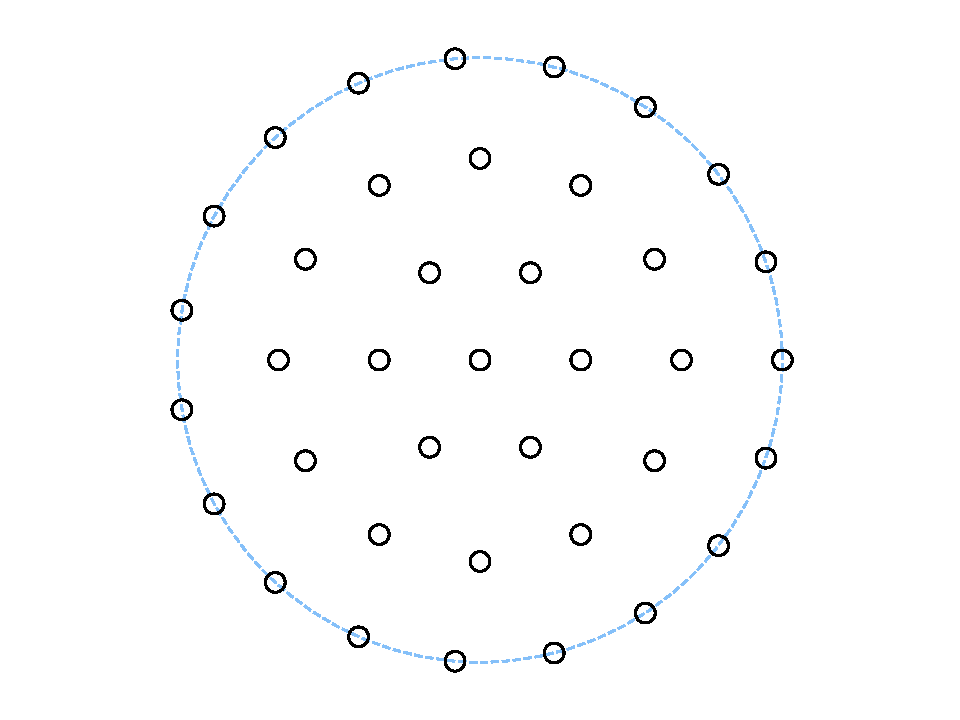
\includegraphics[width=\textwidth, trim={1.5cm, 0cm, 1.5cm, 0cm}, clip]{final_images/layouts/38_turb_start.pdf}
		\caption{Baseline wind farm layout for cases 2 and 3. The circles marking turbine locations are to scale, with diameters equal to the rotor diameter.}
		\label{fig:layout2and3}
	\end{minipage} \hspace{1pc}
	\begin{minipage}[t]{18pc}
		\centering
		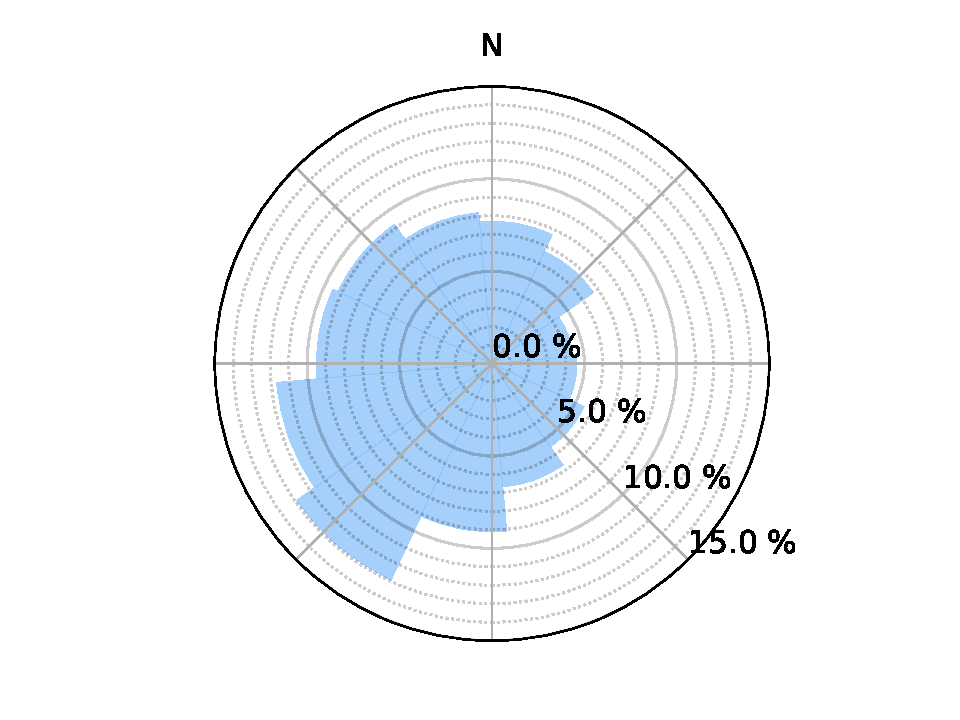
\includegraphics[width=\textwidth, trim={1.5cm 0cm 1.5cm 0cm}, clip]{final_images/windroses/freqwindrose_12_dir.pdf}
		\caption{Directional probability wind rose for case 2. This is the Nantucket wind rose binned into 12 directions \cite{wrcc2017}.}
		\label{fig:freqwindrose_12dir}
	\end{minipage}
\end{figure}

The optimization problem for case 2 was formulated as
%
\begin{equation}\label{eq:case2}
	\begin{aligned} [b]
	\underset{x_i,y_i}{\textrm{maximize}} \quad & AEP(x_i,y_i)~~i=1...38\\
	\textrm{subject to} \quad & s_{ij} \geq 2\*d~~i,j=1...38~~i \neq j\\
	 & [x_c-x_i]^2+[y_c-y_i]^2 \leq r_{b}^2~~i=1...38
	\end{aligned}
\end{equation}
%
In \cref{eq:case2}, $(x_c,y_c)$ is the location of the center of the wind farm, and $r_b$ is the radius of the wind farm boundary. Case 2 has a total of 76 variables and 741 constraints.

\subsection{Case 3: 38 Turbines and 36 Wind Directions}
%
Case 3 is the same as case 2 but with more wind directions and different wind speeds in each direction. We used the Nantucket wind rose binned into 36 directions with the wind speed for each direction determined as the average of all samples in that sector as shown in \cref{fig:speedwindrose_36dir,fig:freqwindrose_36dir}. The optimization problem for case 3 was formulated as shown in \cref{eq:case2} with the same number of variables and constraints.
%
\begin{figure}[h!]
	\centering
	\begin{minipage}[t]{18pc}
		\centering
		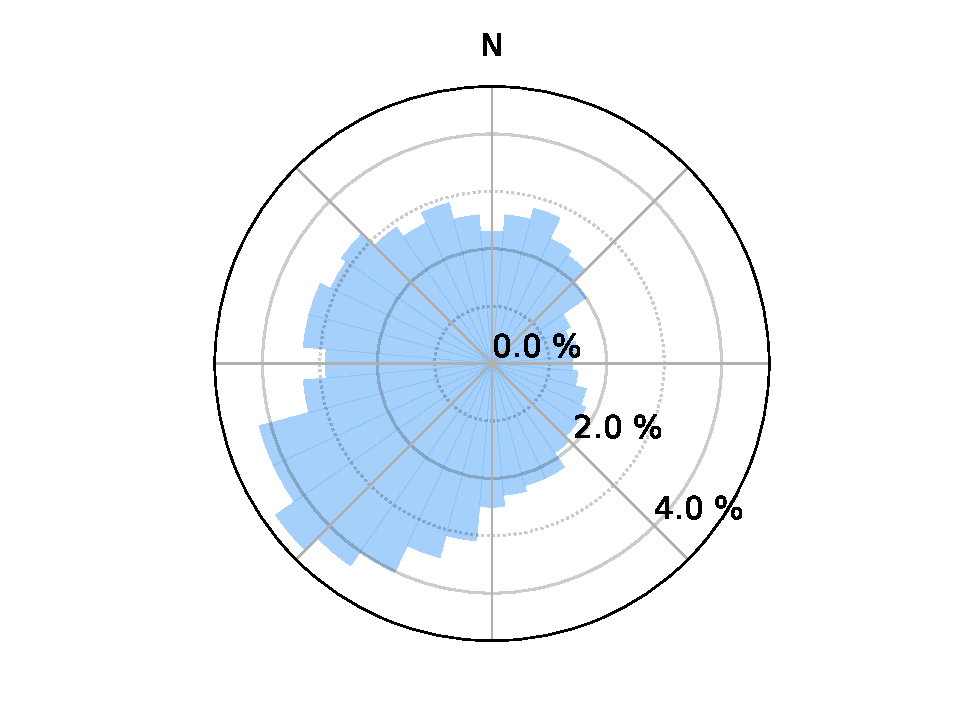
\includegraphics[width=\textwidth, trim={1.5cm 0cm 1.5cm 0cm}, clip]{final_images/windroses/freqwindrose_36_dir.pdf}
		\caption{Directional probability wind rose for case 2. This is the Nantucket wind rose binned into 36 directions \cite{wrcc2017}.}
		\label{fig:freqwindrose_36dir}
	\end{minipage} \hspace{1pc}%
	\begin{minipage}[t]{18pc}
		\centering
		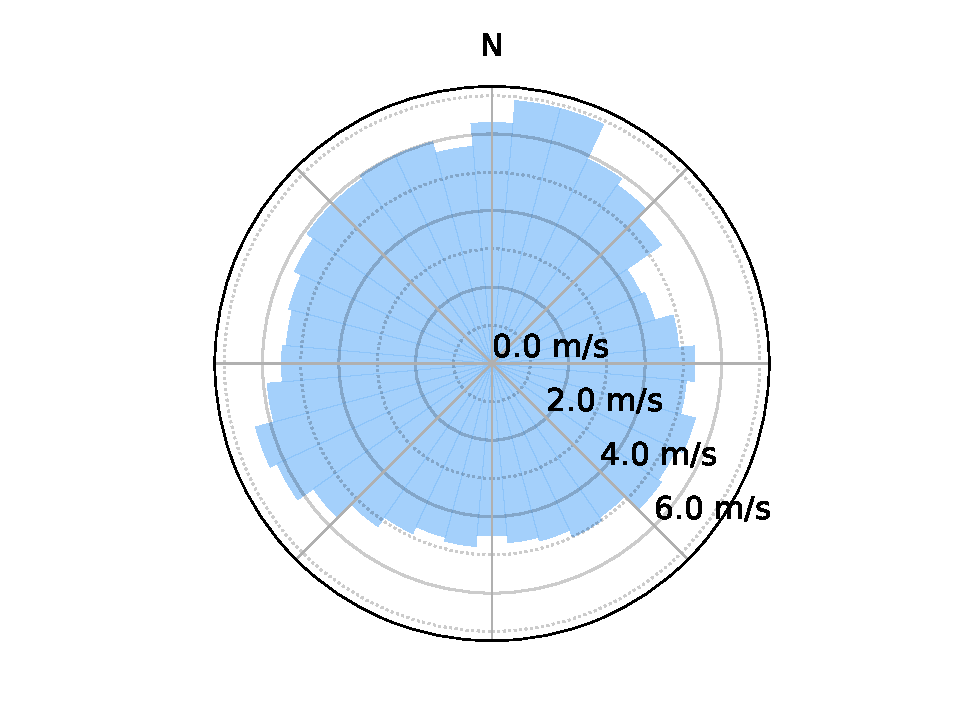
\includegraphics[width=\textwidth, trim={1.5cm, 0cm, 1.5cm, 0cm}, clip]{final_images/windroses/speedwindrose_36_dir.pdf}
		\caption{Average speed wind rose for case 2. This is the Nantucket wind rose binned into 36 directions \cite{wrcc2017}}
		\label{fig:speedwindrose_36dir}
	\end{minipage}
\end{figure}

\subsection{Case 4: 60 Turbines and 72 Wind Directions}
Case 4, based on the Princess Amalia Wind Park, was selected to provide a larger and somewhat more realistic problem. The Amalia wind farm has 60 wind turbines. We used the convex hull of the existing turbine locations to create the boundary \cref{fig:layout4}. We binned wind data into 72 wind directions with wind speed for each direction determined as the average of all samples in that sector as shown in \cref{fig:speedwindrose_72dir,fig:freqwindrose_72dir}.
\begin{figure}[h!]
	\centering
	\begin{minipage}[t]{18pc}
		\centering
		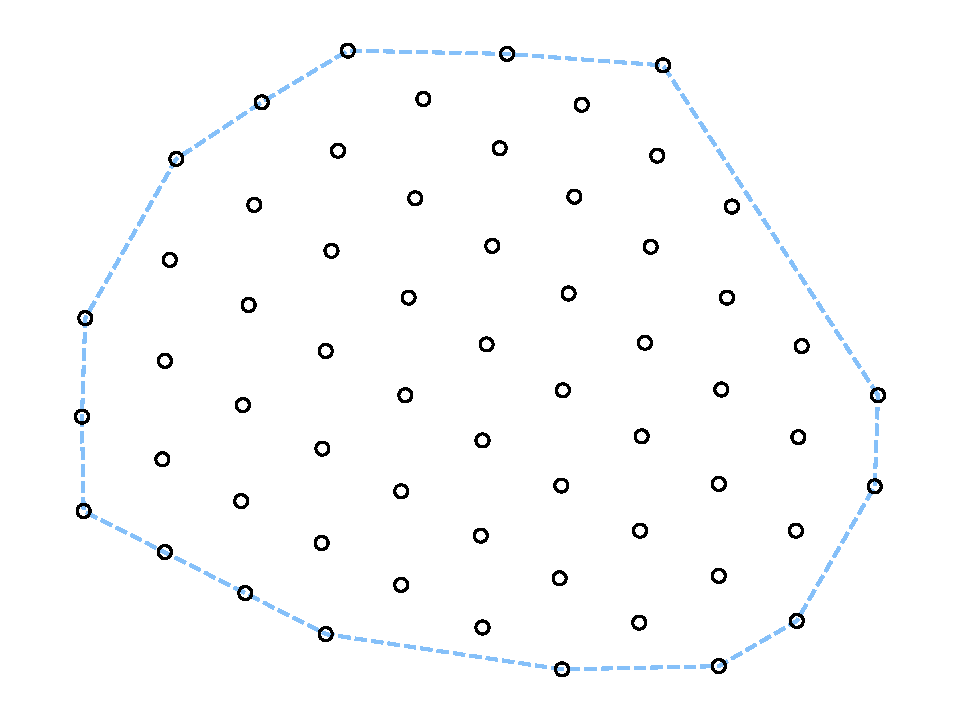
\includegraphics[width=1.\textwidth, trim={1.0cm, 0cm, 1.0cm, 0cm}, clip]{final_images/layouts/60_turb_start.pdf}
		\caption{Baseline wind farm layout for case 4. The circles marking turbine locations are to scale, with diameters equal to the rotor diameter.}
		\label{fig:layout4}
	\end{minipage}\hspace{1pc}%
\end{figure}

\begin{figure}[h!]
	\centering
	\begin{minipage}[t]{18pc}
		\centering
		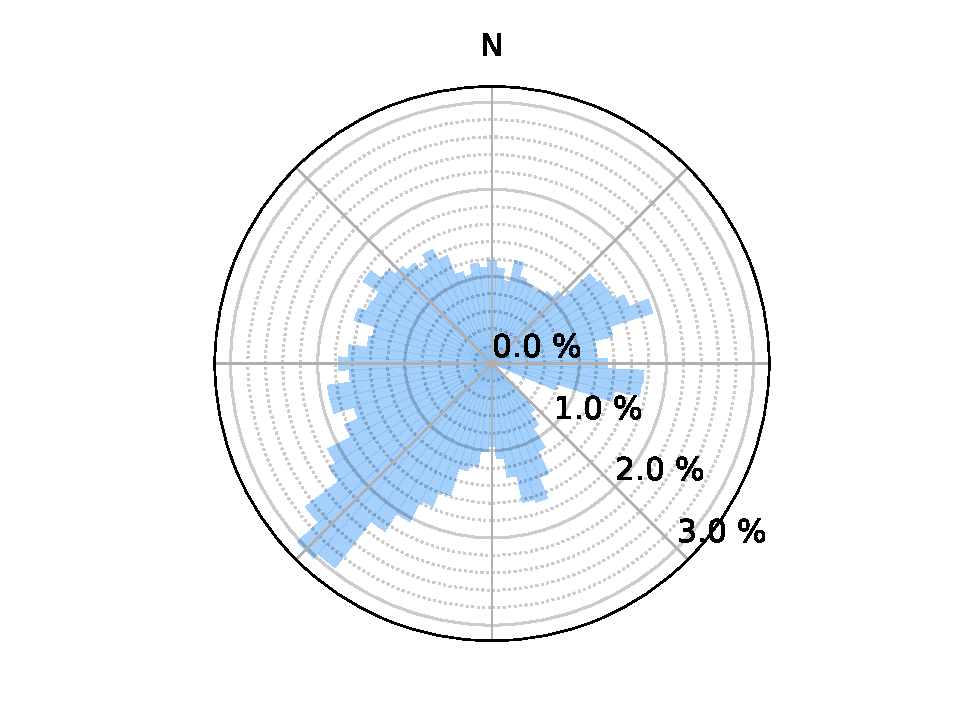
\includegraphics[width=\textwidth, trim={1.5cm 0cm 1.5cm 0cm}, clip]{final_images/windroses/freqwindrose_72_dir.pdf}
		\caption{Direction probability wind rose for case 4. The wind rose is comprised of data from \cite{noordzeewind2006}. Measurements were taken from July 1, 2005, to June 30, 2006.}
		\label{fig:freqwindrose_72dir}
	\end{minipage} \hspace{1pc}%
	\begin{minipage}[t]{18pc}
		\centering
		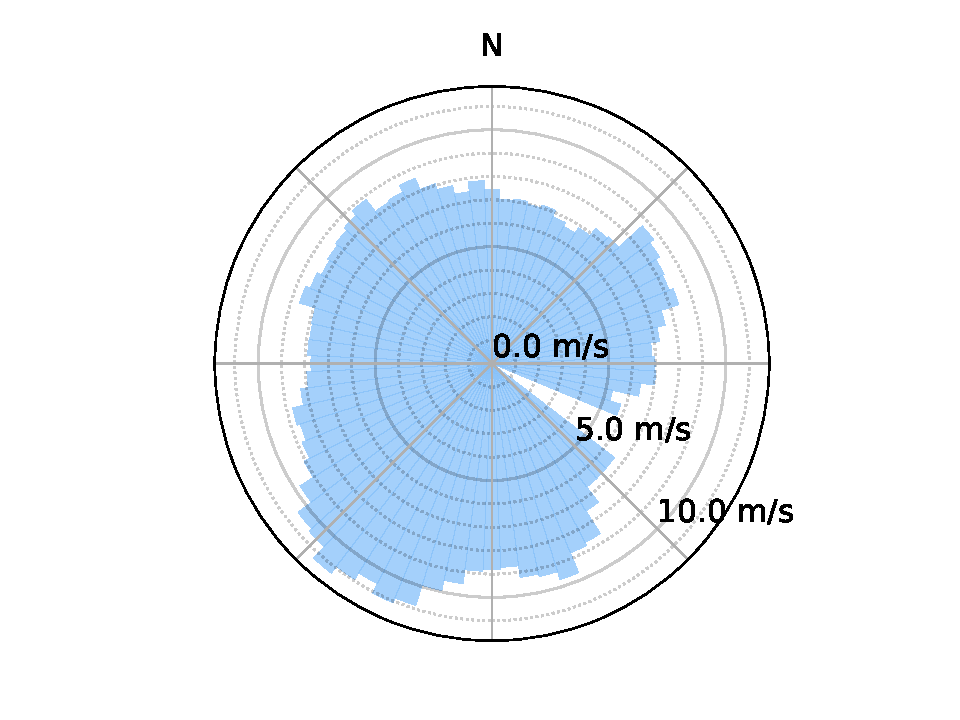
\includegraphics[width=1.\textwidth, trim={1.5cm, 0cm, 1.5cm, 0cm}, clip]{final_images/windroses/speedwindrose_72_dir.pdf}
		\caption{Average speed wind rose for case 4. The wind rose is comprised of data from \cite{noordzeewind2006}. Measurements were taken from July 1, 2005, to June 30, 2006.}
		\label{fig:speedwindrose_72dir}
	\end{minipage}
\end{figure}
%
For case 4, the optimization problem was formulated as shown in \cref{eqn:opt3}
%
\begin{equation}
\label{eqn:opt3}
\begin{aligned} [b]
\underset{x_i,y_i}{\textrm{maximize}} \quad & AEP(x_i,y_i)~~i=1...60\\
\textrm{subject to} \quad & s_{ij} \geq 2\*d~~i,j=1...60,~~i \neq j\\
& b_{ik} \geq 0 ~~ i=1...60, k=1...14
\end{aligned}
\end{equation}
%
Where $b_{i,k}$ represents the distance of each turbine $i$ from each boundary $k$. Case 4 has a total of 120 variables and 2610 constraints.

\section{Implementation Details and Optimization Algorithms}\label{sec:computation}
The code for each wake model was written in Fortran and wrapped in python. In this work, optimization problems were set up and solved in OpenMDAO \cite{gray2010_OpenMDAO} using two optimization algorithms, the gradient-based Sparse Nonlinear OPTimizer (SNOPT)  \cite{gill2005} and the gradient-free Augmented Lagrangian Particle Swarm Optimizer (ALPSO) \cite{jansen2011_alpso}. Both algorithms were used through pyOptSparse \cite{perez2012a}. We obtained exact gradients for both wake models using algorithmic differentiation provided by Tapenade \cite{tapenade2013}.

\section{Tuning the Optimization Methods}\label{sec:tuning}

\subsection{SNOPT}
We used two optimizations for each run with SNOPT when using the Bastankhah model. The first run did not use local turbulence intensity; the second one did. SNOPT was run with different convergence tolerances for each case. Tolerances were determined based on the tolerance required to achieve the majority of the improvement in several test runs without unnecessarily delaying termination. Convergence tolerances used in each case are presented in \cref{tab:snopttols}. The objective and constraint derivatives for all cases were scaled to be between $\pm1$. The objective function was formulated in kWh and was subsequently scaled by $1\times10^{-4}$ for optimization with SNOPT.
%
\begin{table}[h!]
	\centering
	\caption{SNOPT Tolerances And Scaling for Each Case Study}
	\label{tab:snopttols}
	\begin{tabular}{lrrr}
		\toprule
		{} & \multicolumn{2}{c}{Bastankhah } & Jensen Cosine \\
		\cmidrule(lr){2-3} \cmidrule(lr){4-4}
		 & Without Local TI & With Local TI &  \\
		\cmidrule(lr){2-3} 
		Case 1 &  $1\times10^{-2}$ & $1\times10^{-3}$ & \\
		Case 2 & $9\times10^{-3}$ & $1\times10^{-3}$ & $1\times10^{-3}$ \\
		Case 3 & $9\times10^{-3}$ & $1\times10^{-3}$ & \\
		Case 4 &  $1\times10^{-3}$ & $1\times10^{-4}$ &  \\
		\bottomrule
	\end{tabular}
\end{table}

\subsection{ALPSO} 
ALPSO was run using the default parameters provided in pyOptSparse \cite{wu2020} with a few exceptions. First, the craziness velocity was set to be $1\times10^{-2}$ as this value resulted in increased optimized AEP compared to the default value across all the cases we tested. We tried adjusting the initial particle velocity, but found no difference in results. As demonstrated in \cite{jansen2011_alpso}, we tested a series of values for inner iteration number and found that the inner iteration count had a large impact on the end results and convergence rates for all cases tested. We used different inner iteration counts for each case study, but held the number of function calls relatively constant at about $2\times 10^4$ as all cases appeared converged after this many function calls regardless of the number of inner iterations. We used a constant population seed of 1.0 while testing inner iteration counts and a random seed for the final case study results. The number of outer iterations was determined based on the number inner iterations and desired function call cap for each case. The ALPSO convergence history for each case study with varied inner iteration counts is shown in \cref{fig:alpso-ii-16-20,fig:alpso-ii-38-12,fig:alpso-ii-38-36,fig:alpso-ii-60-72}. The objective and design variables were all scaled to be between -1 and 1.  All optimization runs using ALPSO had a population size of 30. The adjusted meta-parameters used for the various ALPSO runs are shown in \cref{tab:alpsoparams}.

\begin{figure}[htp]
	\centering
	\begin{minipage}[t]{0.48\textwidth}
		\centering
		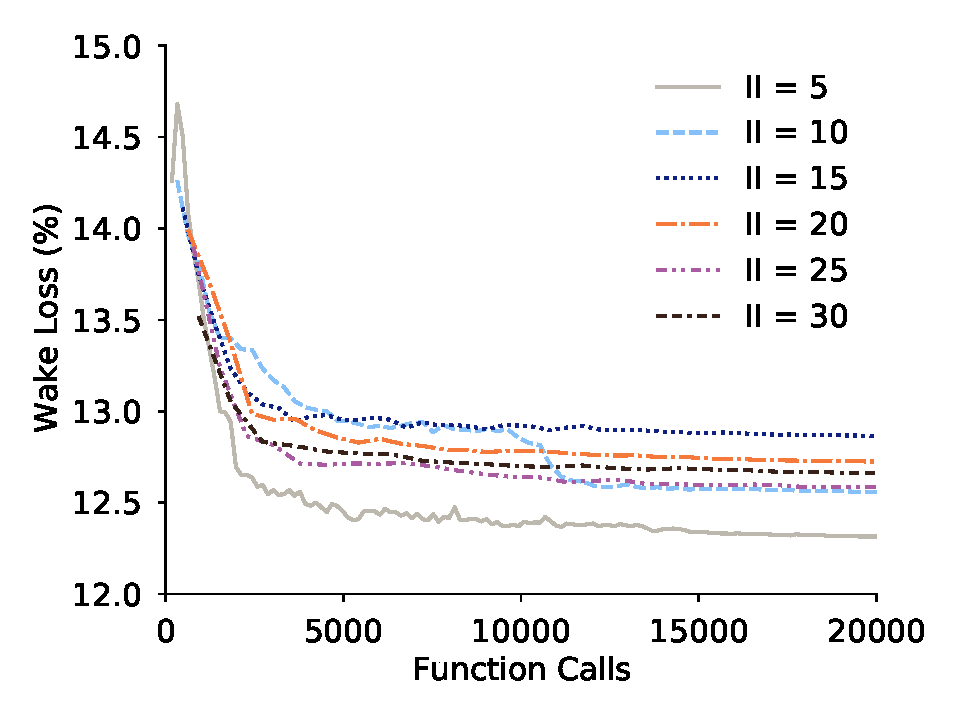
\includegraphics[width=\textwidth, trim={0cm 0cm 0cm 0cm}, clip]{tests/alpso_test_16turbs_20dirs.pdf}
		\caption{Comparing ALPSO convergence history for 16 turbines, 20 directions, and varying numbers of inner iterations.}
		\label{fig:alpso-ii-16-20}
	\end{minipage}\hspace{1pc}%
	\begin{minipage}[t]{0.48\textwidth}
		\centering
		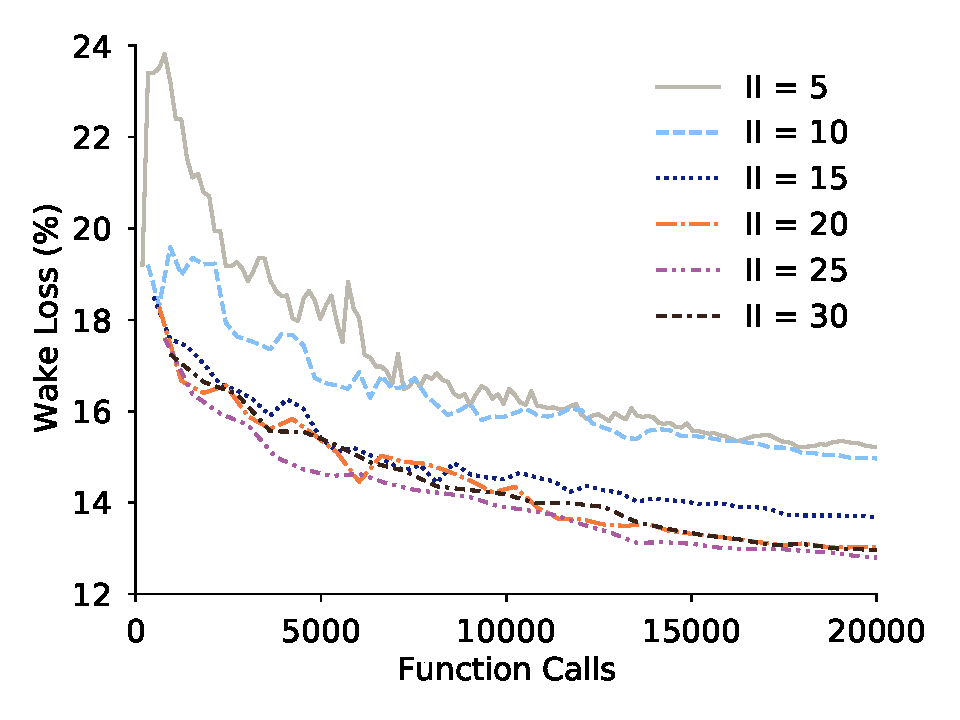
\includegraphics[width=\textwidth]{tests/alpso_test_38turbs_12dirs.pdf}
		\caption{Comparing ALPSO convergence history for 38 turbines, 12 directions, and varying numbers of inner iterations.}
		\label{fig:alpso-ii-38-12}
	\end{minipage} 
\end{figure}
\begin{figure}[htp]
	\centering
	\begin{minipage}[t]{0.48\textwidth}
		\centering
		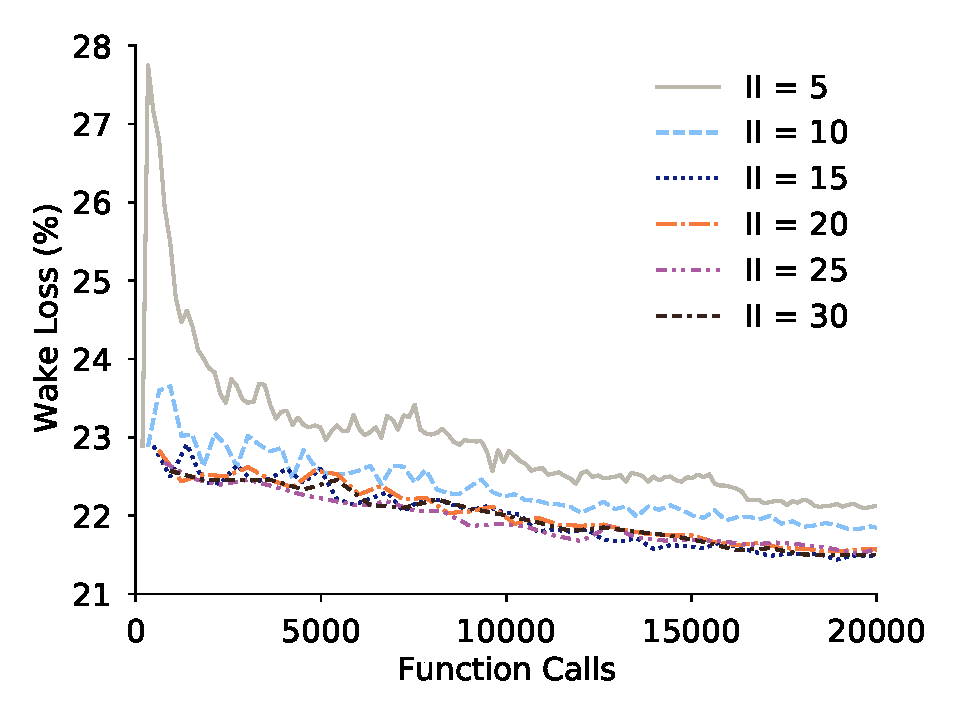
\includegraphics[width=\textwidth, trim={0cm 0cm 0cm 0cm}, clip]{tests/alpso_test_38turbs_36dirs.pdf}
		\caption{Comparing ALPSO convergence history for 38 turbines, 36 directions, and varying numbers of inner iterations.}
		\label{fig:alpso-ii-38-36}
	\end{minipage}\hspace{1pc}%
	\begin{minipage}[t]{0.48\textwidth}
		\centering
		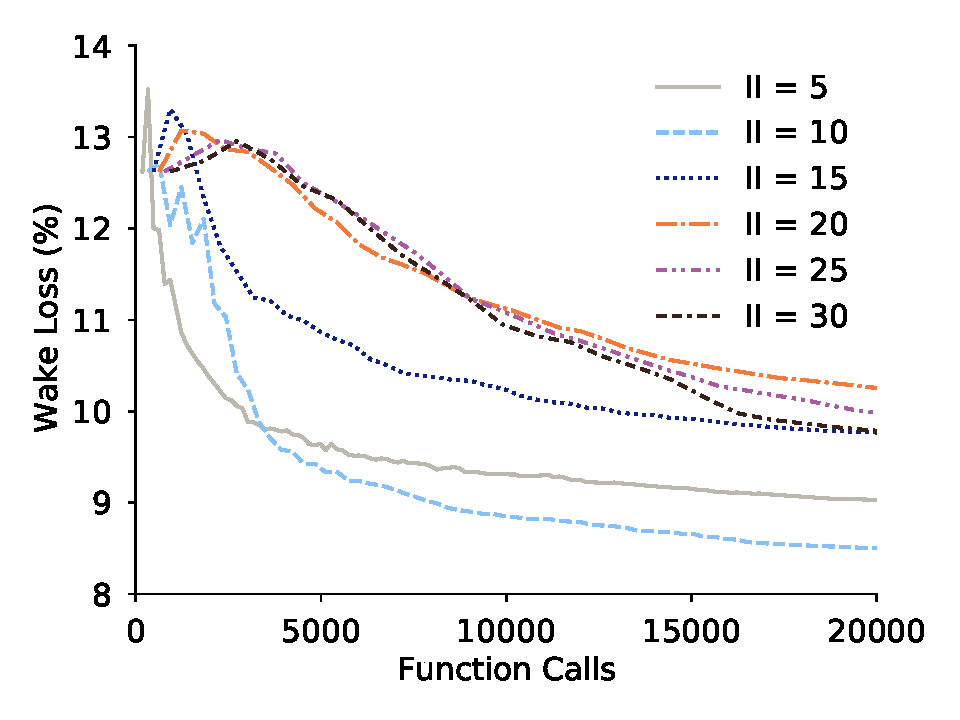
\includegraphics[width=\textwidth]{tests/alpso_test_60turbs_72dirs.pdf}
		\caption{Comparing ALPSO convergence history for 60 turbines, 72 directions, and varying numbers of inner iterations.}
		\label{fig:alpso-ii-60-72}
	\end{minipage} 
\end{figure}

\begin{table}[h!]
	\centering
	\caption{Varied ALPSO Meta-Parameters}
	\label{tab:alpsoparams}
	\begin{tabular}{lrrr}
		\toprule
		{} & Inner Iterations & Outer Iterations & Function Calls\\
		\cmidrule(lr){2-4}
		Case 1 &  5  & 134 & 20130 \\
		Case 2 & 25 & 28  & 21030 \\
		Case 3 & 15 & 45 & 20280 \\
		Case 4 & 10 & 68 & 20430 \\
		\bottomrule
	\end{tabular}
\end{table}

While it may be noted that each optimization run with ALPSO is similar to running 30 optimizations using a gradient-based algorithm in population size, we decided to run a full set of 200 optimizations for each test, just as was done for SNOPT. This decision was to reflect how optimizations are often performed in practice, with many optimizations being run regardless of the algorithm being used. While ALPSO and other population-based algorithms do carry many samples of the design space concurrently, they are used to inform one another and drive to a single final solution, playing a similar role as the gradients do in gradient-based optimization. We considered a direct comparison between full optimizations, rather than population members, to be more informative in how results would look in practice using each algorithm. This approach also enables a direct comparison of function calls and the optimization objective.

\subsection{SNOPT+WEC}\label{sec:bpa_wec_comparison}

We compared the performance of WEC-A, WEC-D, and WEC-H with the Bastankhah  model by varying both the number of intermediate optimizations (steps) to run and the maximum values of the WEC factor ($\xi$ or $\theta_\xi$) to use. To investigate the WEC methods and parameter selection, we used Case 2 as discussed in \cref{sec:case2}. When the maximum WEC factor value was varied, the number of steps was held at six. When the number of steps was varied, the maximum WEC factor was held at $\theta_\xi = 9 ^\circ$, $\xi=3$, and $\xi=3$, for WEC-A, WEC-D, and WEC-H respectively. All 200 starting layouts were tested with each parameter set. For comparing the wake expansion methods, the $k^*$ value in \cref{eq:kstar} was not adjusted to the local turbulence intensity during optimization, but was adjusted for calculating the results shown.

The mean wake loss results for the various wake spreading approaches are provided in \cref{fig:aepmean-wm,fig:aepmean-ws}. Here we see that, on average, WEC-D results in less wake loss with a WEC value of 3 and using 5 or more steps, while WEC-A has its lowest average wake loss for a maximum WEC angle of $6^\circ$, and WEC-H minimizes average wake loss most with lower WEC values. On average, wake loss minimized using WEC-A or WEC-H does not appear to be impacted by changing the number of steps.
%
\begin{figure}[ht]
	\centering
	\begin{minipage}[t]{0.47\textwidth}
		\centering
		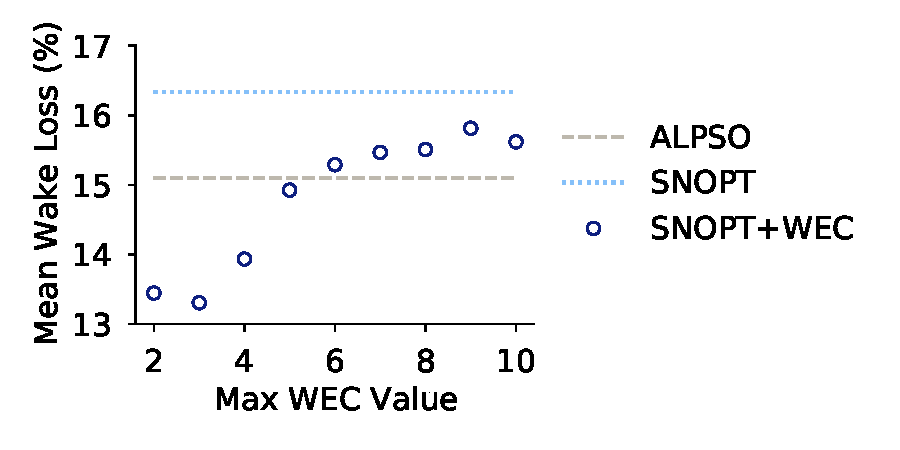
\includegraphics[width=\textwidth, trim={0cm 0cm 0cm 0cm}, clip]{tests/maxwec_const_nsteps6_mean}
		\caption{Mean wake loss results for varying the maximum WEC expansion parameter while holding the number of steps constant at six. Each data point represents 200 separate optimizations with different starting points. Note: the WEC value and WEC angle axes are not directly comparable.}
		\label{fig:aepmean-wm}
	\end{minipage}\hspace{1pc}
	% Figure displaying results from aep vs crosswind position tests for Jensen
	\begin{minipage}[t]{0.47\textwidth}
		\centering
		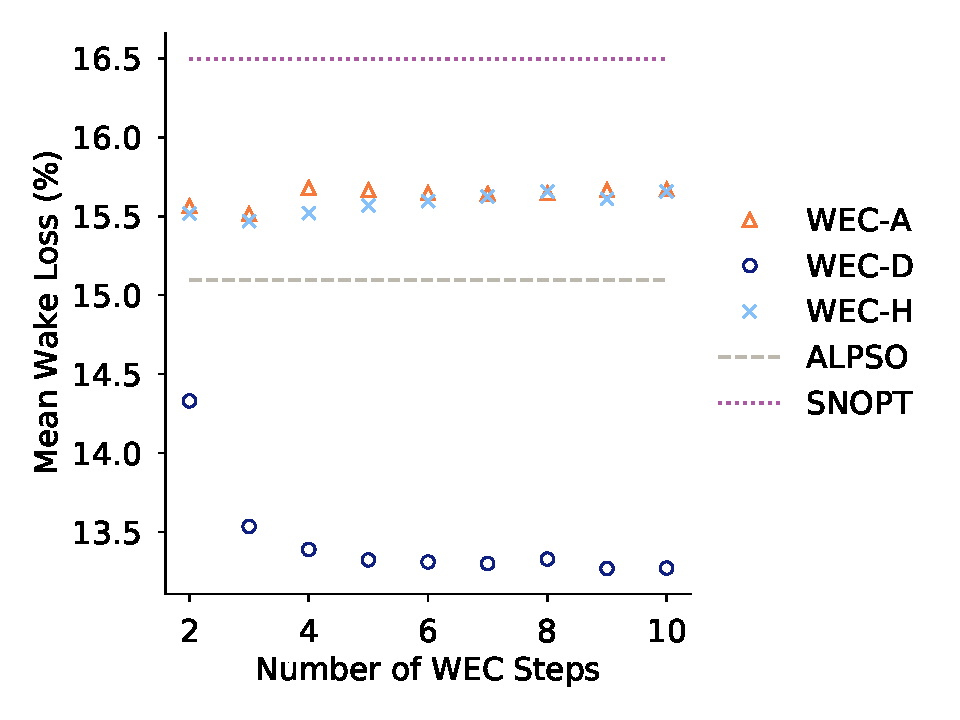
\includegraphics[width=\textwidth]{tests/nsteps_const_maxwec_mean}
		\caption{Mean wake loss results for varying the number of WEC steps while holding the expansion parameter constant at three. Each data point represents 200 separate optimizations with different starting points.}
		\label{fig:aepmean-ws}
	\end{minipage}
\end{figure}

We found that the minimum wake loss is achieved when the maximum WEC angle is $9^\circ$ for WEC-A and when the maximum WEC value is 3 for WEC-D and WEC-H. There does not appear to be a clear relationship between minimum wake loss and number of steps for WEC-A or WEC-H. WEC step numbers greater than or equal to 3 achieve approximately equal minimum wake loss for WEC-D and WEC-H individually, but on average WEC-D performs much better than either WEC-A or WEC-H.

The lowest standard deviations occur when the WEC angle is $5^\circ$ for WEC-A, the WEC value is 3 for WEC-D, and when the WEC value is 2 for WEC-H. There is no clear relationship between number of steps and the standard deviation for WEC-A and WEC-H, but we found it best to use at least 4 or 5 steps with WEC-D to achieve a small standard deviation (meaning more consistent results).

We determined that the WEC-D method is the best wake spreading method we investigated as it had the lowest minimum, mean, and standard deviation of wake loss. We decided to use WEC-D with 6 steps and a maximum $\xi$ value of three for the case studies. The better performance of WEC-D over WEC-A and WEC-H can be explained by the fact that both WEC-A and WEC-H alter the wake shape, while WEC-D only multiplies the standard deviation of the basis functions in a manner consistent with Gaussian continuation optimization theory as discussed in \cite{mobahi2015}. In the balance of this paper we will refer to WEC-D as WEC because the other variants are not relevant in the remainder of this discussion. 

When optimizing with WEC in the case studies, we adjusted the convergence tolerances because the WEC steps are primarily for exploration and escaping local optima. The corresponding convergence tolerances and WEC values used at each step with SNOPT+WEC are shown in \cref{tab:wectols}. 

\begin{table}[h!]
	\centering
	\caption{WEC Parameters and Convergence Tolerances}
	\label{tab:wectols}
	\begin{tabular}{lrrrrrrr}
		\toprule		
	WEC step & 1 & 2 & 3 & 4 & 5 & 6 & Final \\
	\cmidrule{2-8}
	WEC Value ($\xi$) & 3.0 & 2.6 & 2.2 & 1.8 & 1.4 & 1.0 & 1.0 \\
	Local TI & No & No & No & No & No & No & Yes \\
	Case 1 &	$1\times10^{-2}$ & $1\times10^{-2}$ & $1\times10^{-2}$ & $1\times10^{-2}$ & $1\times10^{-2}$ & $1\times10^{-2}$ & $1\times10^{-3}$ \\
	Cases 2-4 &	$9\times10^{-3}$ & $9\times10^{-3}$ & $9\times10^{-3}$ & $9\times10^{-3}$ & $9\times10^{-3}$ & $9\times10^{-3}$ & $1\times10^{-3}$ \\
		\bottomrule
	\end{tabular}
\end{table}

\subsection{ALPSO+WEC}
Because WEC adjusts the design space, it can be applied with any optimization algorithm. To see if WEC is helpful for gradient-free algorithms, we tested the impact of WEC with ALPSO in case 2 (see \cref{sec:case2}). For this test we used only WEC-D and used a maximum WEC value of 3 with 6 steps, the same maximum $\xi$ value and number of steps that we found to be best for using WEC with SNOPT. The objective and constraints were all scaled to be between $\pm1$. We chose to use 25 inner iterations, the number of inner iterations that was best for ALPSO without WEC. The WEC steps were applied by dividing the outer iterations by the number of WEC steps plus 1 and rounding up, so each WEC step was run with 5 outer iterations. The WEC steps were run with no local TI, just as for WEC with SNOPT, and a final 5 outer iterations was run with local TI. It is likely that there are more optimal settings for using WEC with ALPSO, such as tuning the number of inner and outer iterations for the changing design spaces at each WEC step. When using WEC with SNOPT, most of the turbine movement tends to occur during the first WEC step. It seems reasonable then that using more outer iterations in the first WEC step with ALPSO may lead to better results because the early part of the optimization is when most of the exploration takes place and the highest WEC value provides the most reduction in local optima. However, this case was only performed as a basic test to see if there was any significant benefit for applying WEC while optimizing with ALPSO and so parameter values were based on what we learned from the preceding tuning studies.

\subsection{WEC with the Jensen Cosine Model}
As a proof of concept in applying WEC to other wake models, we implemented WEC with the Jensen cosine model using the same maximum value of $\xi$ (3) and the same number of WEC steps (6) as found best for use with WEC as applied to the Bastankhah model in \cref{sec:bpa_wec_comparison}. We tested WEC with the Jensen cosine model only on case 2 (38 turbines and 12 directions. See \cref{sec:case2}). Further improvements with WEC are likely available if WEC were tuned to this model and case combination.

\section{Results and Discussion}\label{sec:results}

In the WFLO problem, we  want low wake loss values, tight distributions, and relatively few function calls. The benefit of low wake loss is increased efficiency, leading to a reduced cost of energy. Tight distributions indicate that results are more consistent and less dependent on the starting layout, so we should need fewer optimizations to be confident of having a good wind farm design. A low number of function calls shows that wind farm design optimization can be done more quickly, more variables could be tested, and planning costs could be reduced. WEC generally reduces the variance and value of wake loss while keeping function calls well below the number required for gradient-free optimization. Starting and final wake loss distributions for the case studies are shown in the box plots of \cref{fig:boxplots}. 
%
\begin{figure}[h!]
	\centering
	\begin{minipage}[t]{\textwidth}
		\centering
		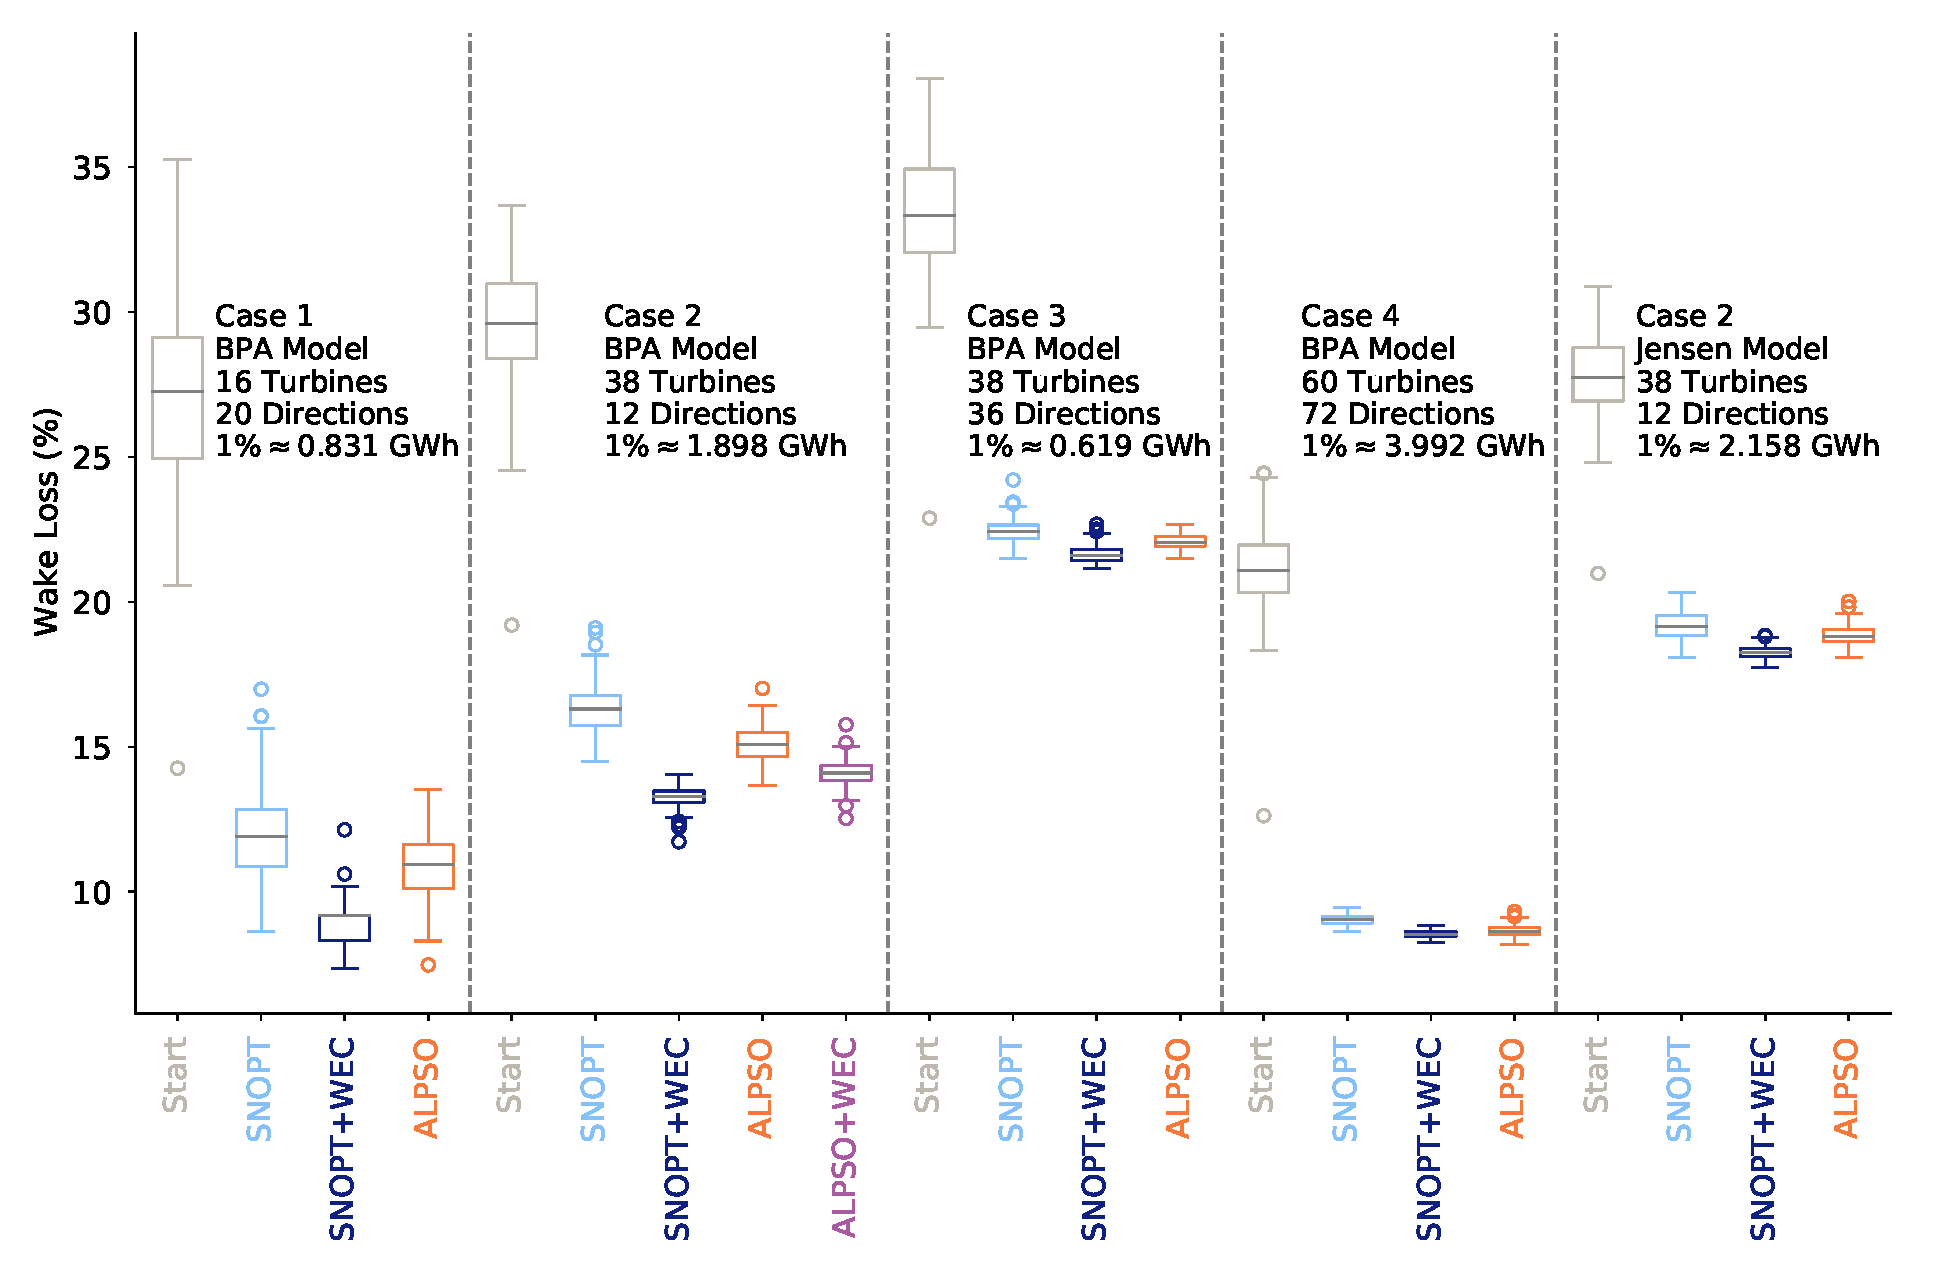
\includegraphics[width=\textwidth]{final_images/results/dist_boxpercentwakeloss.pdf}  
		\caption{Results distributions of all case studies.}
		\label{fig:boxplots}
	\end{minipage} 
\end{figure}

We can see in \cref{fig:boxplots} that all the optimization methods applied were successful at finding fairly good results, but it is clear that WEC has a significant impact, reducing the mean, minimum, and standard deviation of the wake loss distributions for all cases as compared with SNOPT or ALPSO alone, with the exception that ALPSO found the best overall result for case 4 . However, SNOPT+WEC  provided the best results on average for all cases. While most of the distributions are fairly normally distributed, the WEC results for case 1 did have some high outliers. It is also clear that WEC improved the results of ALPSO on case 2 on average and in finding a better overall solution. The impact of WEC with ALPSO was less than the impact of WEC with SNOPT. For case 2, the SNOPT+WEC distribution does not even overlap with the SNOPT distribution. The low outliers in the starting location wake loss distributions are the designed layouts depicted in \cref{fig:layout1,fig:layout2and3,fig:layout4}.

The convergence history for SNOPT, SNOPT+WEC, and ALPSO for each case study are shown in \cref{fig:case-1-histories,fig:case-2-histories,fig:case-2j-histories,fig:case-3-histories,fig:case-4-histories}. The ALPSO runs all terminated with the same number of function calls because function calls was controlled by the number of inner and outer iterations (see \cref{tab:alpsoparams}). The straight lines in the ALPSO histories (from $1\times10^0$ to about $1.5\times10^2$ in \cref{fig:case-1-histories}) represent the first outer iteration because we have only plotted ALPSO and ALPSO+WEC points at the completion of each outer iteration. This pattern is seen in the ALPSO and ALPSO+WEC convergence histories for all of the case studies. Straight lines can also be seen in the SNOPT and SNOPT+WEC convergence histories in each of the case studies. These are just small steps taken that appear to have no change in the figures. We have adjusted wake loss values to be calculated by the wake models without WEC and with local TI if applicable in all the convergence history figures. This way we can see what is happening in the design space we are interested in, rather than the altered design space used to inform the optimization algorithms. The y-axes in \cref{fig:case-1-histories,fig:case-2-histories,fig:case-2j-histories,fig:case-3-histories,fig:case-4-histories} correspond with the y-axis in \cref{fig:boxplots}, but with bounds adjusted as appropriate for visualizing the convergence histories of each case study. We chose to use a log scale for function calls because of the large difference in the number of function calls used for gradient-based methods compared to the number of function calls used for the gradient-free methods. The median number of function calls differed by one to two orders of magnitude (see \cref{tab:case1,tab:case2,tab:case2jensen,tab:case3,tab:case4}).

\begin{figure}[h!]
	\centering
	\begin{minipage}[t]{.45\textwidth}
		\centering
		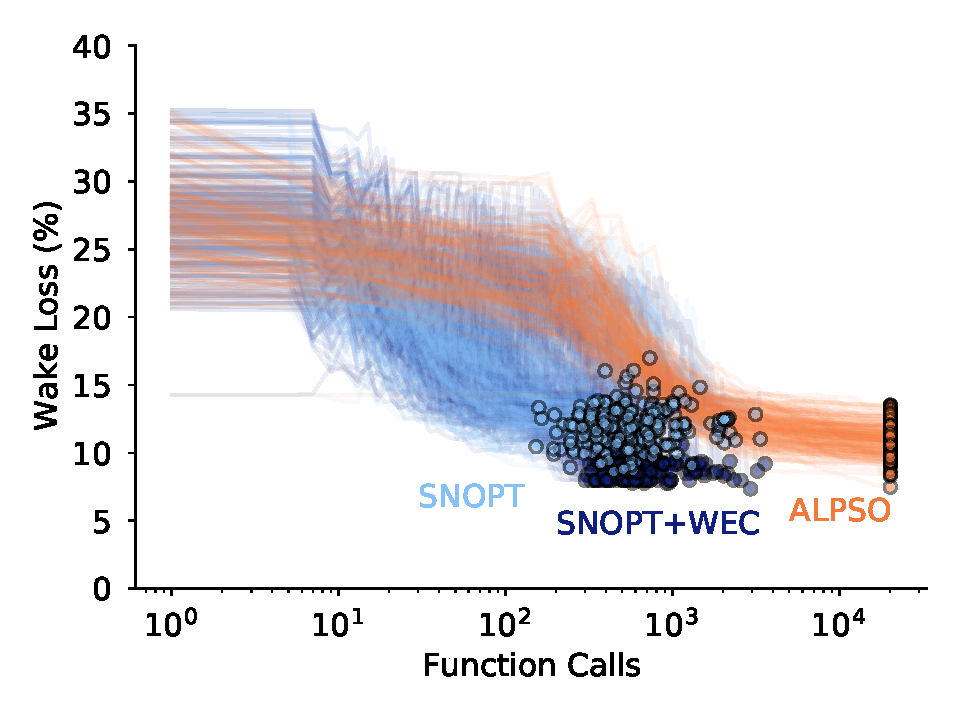
\includegraphics[width=\textwidth]{final_images/results/convergence_history_BPAmodel_16turbs_20dirs}  
		\caption{Convergence histories of optimizations for case 1 (16 turbines and 20 wind directions) using the Bastankhah model. Markers indicate optimized values.}
		\label{fig:case-1-histories}
	\end{minipage}
\end{figure}

The convergence histories for case 1, shown in \cref{fig:case-1-histories}, illustrate the significant drop in wake loss due to using WEC with only a small extra cost in function calls compared to SNOPT alone. The same effect can be seen in the other cases as shown in \cref{fig:case-2-histories,fig:case-2j-histories,fig:case-3-histories,fig:case-4-histories}. While SNOPT+WEC did terminate in fewer function calls than SNOPT in case 4 (\cref{fig:case-4-histories}), the convergence rate was still higher for SNOPT alone. The rate of convergence was much higher for SNOPT than for ALPSO, with or without WEC, with SNOPT alone nearing convergence within the same number of function calls required for ALPSO to complete a single outer iteration. The convergence rate is also the most noticeable difference between the Bastankhah and Jensen model results. As can be seen in comparing \cref{fig:case-2-histories} and \cref{fig:case-2j-histories}, SNOPT, with or without WEC, generally converges faster when using the Jensen model than when using the Bastankhah model. However, the convergence rate of ALPSO appears quite similar. The difference in convergence rate for the gradient-free algorithm is likely due to the simpler and smoother nature of the Jensen model compared with the Bastankhah model.

Because WEC allows transitions through, and out of, local optima, the wake loss for cases with WEC applied appear to remain at higher levels longer in the convergence histories than without WEC. This is a feature of the method and demonstrates the effectiveness of WEC at allowing optimization algorithms to escape local optima. The different characteristics in the convergence paths with and without WEC, for both SNOPT and ALPSO, are very apparent in \cref{fig:case-2-histories}, where both algorithms with WEC stay higher longer and then drop rapidly below the results of the algorithms without WEC.

\begin{figure}[h!]
	\centering
	\begin{minipage}[t]{.45\textwidth}
		\centering
		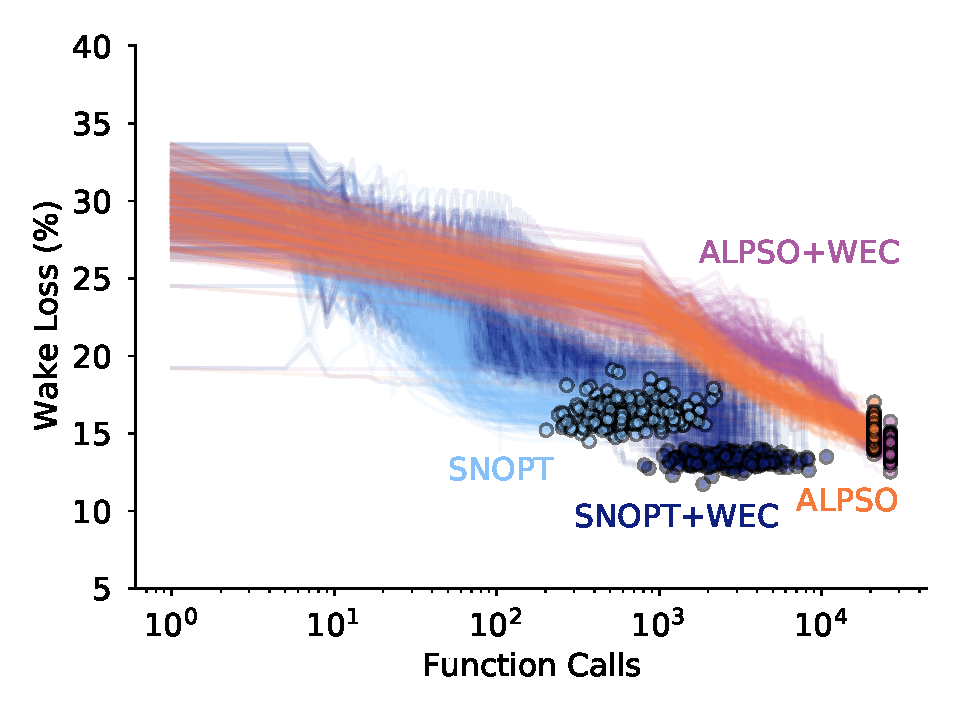
\includegraphics[width=\textwidth]{final_images/results/convergence_history_BPAmodel_38turbs_12dirs}  
		\caption{Convergence histories of optimizations for case 2 (38 turbines and 12 wind directions) using the Bastankhah model. Markers indicate optimized values.}
		\label{fig:case-2-histories}
	\end{minipage}\hspace{1pc}
	\begin{minipage}[t]{0.45\textwidth}
		\centering
		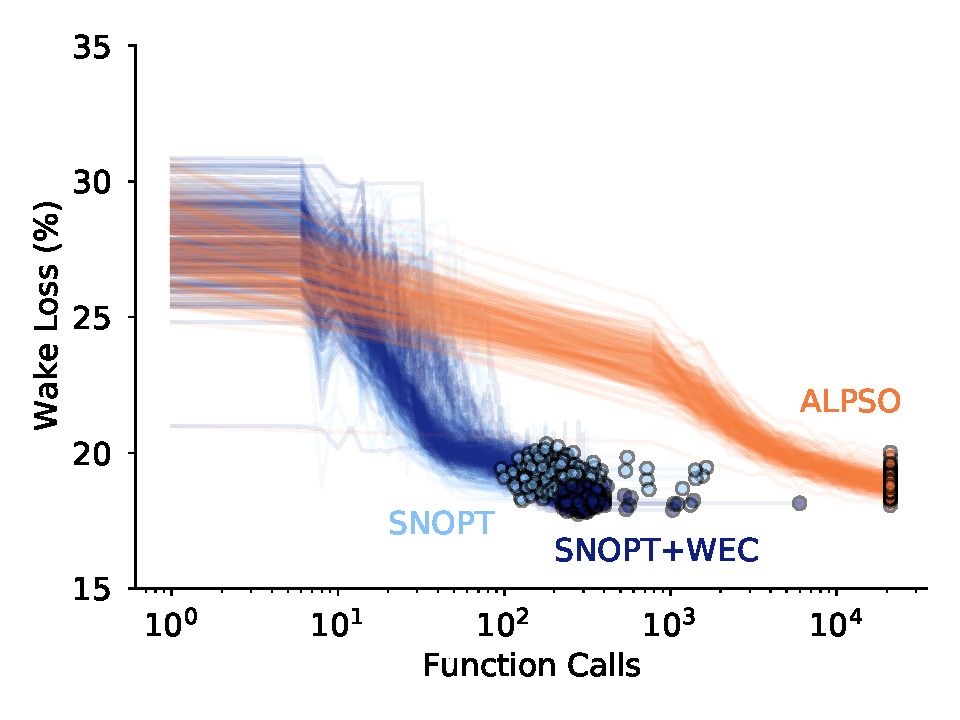
\includegraphics[width=\textwidth]{final_images/results/convergence_history_JENSENmodel_38turbs_12dirs}  
		\caption{Optimization convergence histories for case 2 (38 turbines and 12 wind directions) using the Jensen model. Markers indicate optimized values.}
		\label{fig:case-2j-histories}
	\end{minipage}
\end{figure}

Cases 3 and 4 (\cref{fig:case-3-histories,fig:case-4-histories}) showed similar trends as cases 1 and 2 (\cref{fig:case-1-histories,fig:case-2-histories,fig:case-2j-histories}), but with smaller gains in wake loss for using WEC over not using WEC. Cases 3 and 4 also had wider spreads in the number of function calls required for SNOPT to converge. There are two likely contributors to this difference. The first is an increase in the number of wind directions and different wind speeds in each wind direction for cases 3 and 4. The second is that case 4 provides more space for the turbines in general, resulting in a flatter design space with more similar local optima. The increased wind resource complexity and flatter design space could both increase the number of function calls required. More benefit may also be available from WEC on these cases if WEC were tuned specifically to them. Because we tuned only to case 2, we may have missed some potential improvements available through WEC for cases 1, 3, and 4. However, because wake loss is relative to the energy available, the actual energy gains for using WEC in case 4 are greater than in any of the other cases except case 2 with Bastankhah.  Even without tuning WEC to these cases specifically, the SNOPT with WEC results are significant, and only slightly overlapped, as compared to the SNOPT results without WEC. Using SNOPT+WEC also resulted in the best average for case 4 and the best overall and average for case 3, with SNOPT+WEC giving a result nearly equal to the best found by ALPSO on case 4.

\begin{figure}[h!]
	\centering
	\begin{minipage}[t]{.45\textwidth}
		\centering
		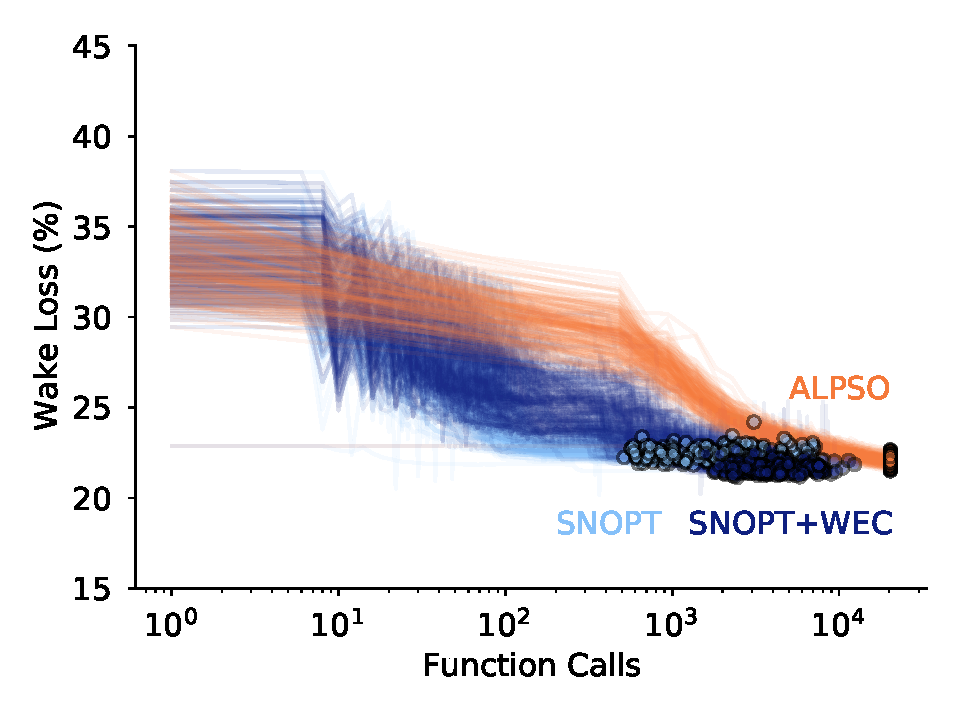
\includegraphics[width=\textwidth]{final_images/results/convergence_history_BPAmodel_38turbs_36dirs}  
		\caption{Convergence histories of optimizations for case 3 (38 turbines and 36 wind directions) using the Bastankhah model. Markers indicate optimized values.}
		\label{fig:case-3-histories}
	\end{minipage} \hspace{1pc}
	\begin{minipage}[t]{.45\textwidth}
		\centering
		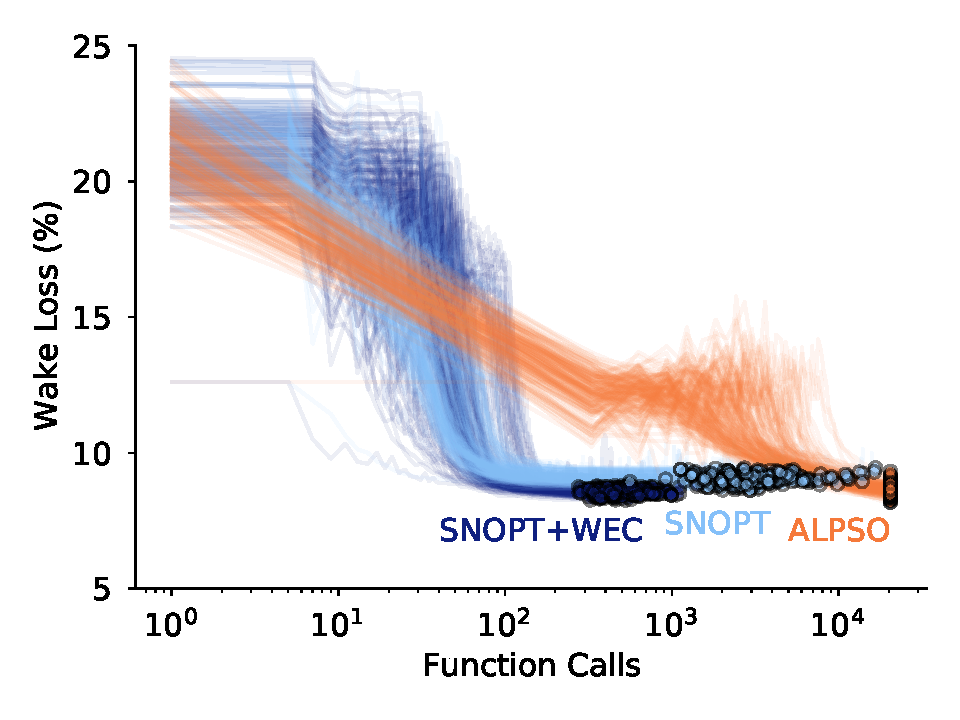
\includegraphics[width=\textwidth]{final_images/results/convergence_history_BPAmodel_60turbs_72dirs}  
		\caption{Convergence histories of optimizations for case 4 (60 turbines and 72 wind direct          ions) using the Bastankhah model. Markers indicate optimized values.}
		\label{fig:case-4-histories}
	\end{minipage} 
\end{figure}

We compared wake loss and the number of function calls required for each of the cases discussed previously. We used function calls as a surrogate for time. We did not report wall time because we did not maintain enough consistency in the computational resources used for each optimization run (cores, processor types, computational isolation, etc). We also performed a Welch's t-test between the SNOPT and SNOPT+WEC wake loss percentage results, as well as between the ALPSO and ALPSO+WEC wake loss percentage results. The Welch's t-tests showed $p<0.001$ for all cases, indicating a high confidence that the results are not a product of random chance. The final statistical results of optimizations from the 200 starting points for each optimization method on the case studies presented in \cref{sec:casestudies} are shown in \cref{tab:case1,tab:case2,tab:case2jensen,tab:case3,tab:case4}. 

 While mean and median are both reported for the final wake loss in each case, they were nearly equal for all cases except for case 1 with SNOPT+WEC. In case 1, the SNOPT+WEC results had high outliers that skewed the mean upward. SNOPT+WEC resulted in the lowest average wake loss percentage across all cases. The largest difference was for case 2, where SNOPT+WEC resulted in a reduction in wake loss percentage of 3.058 compared with the results from SNOPT alone.
 
\begin{table}
	\centering
	\caption{Case 1 Results for Bastankhah Model: 16 Turbines, 20 Directions}
	\label{tab:case1}
	\begin{threeparttable}
	\begin{tabular}{lrrrrrrrrr}
		\toprule
		{} & \multicolumn{3}{c}{Function Calls} & \multicolumn{6}{c}{Wake Loss (\%)\tnote{*}} \\
		\cmidrule(lr){2-4} \cmidrule(lr){5-10}
		{} &         Median &    Low &   High &        Median &   Mean &    SD &   Low &   High &          p \\
		\cmidrule(lr){2-4} \cmidrule(lr){5-10}
		SNOPT     &            546 &    152 &   3348 &        11.898 & 11.882 & 1.470 & 8.630 & 16.988 &            \\
		SNOPT+WEC &            618 &    300 &   3580 &         9.169 &  8.860 & 0.698 & 7.346 & 12.137 &  $< 0.001$ \\
		ALPSO     &          20130 &  20130 &  20130 &        10.951 & 10.940 & 1.094 & 7.479 & 13.523 &            \\
		\bottomrule
	\end{tabular}
	\begin{tablenotes}
		\item[*]For case 1 with Bastankhah, $1\%$ wake loss represents approximately 0.83 GWh
	\end{tablenotes}	
	\end{threeparttable}
\end{table}
\begin{table}
	\centering
	\caption{Case 2 Results for Bastankhah Model: 38 Turbines, 12 Directions}
	\label{tab:case2}
	\begin{threeparttable}
	\begin{tabular}{lrrrrrrrrr}
		\toprule
		{} & \multicolumn{3}{c}{Function Calls} & \multicolumn{6}{c}{Wake Loss (\%)\tnote{*}} \\
		\cmidrule(lr){2-4} \cmidrule(lr){5-10}
		{} &         Median &    Low &   High &        Median &   Mean &    SD &    Low &   High &          p \\
		\cmidrule(lr){2-4} \cmidrule(lr){5-10}
		SNOPT     &            591 &    202 &   2220 &        16.304 & 16.338 & 0.790 & 14.505 & 19.102 &            \\
		SNOPT+WEC &           2679 &    814 &  10696 &        13.285 & 13.280 & 0.341 & 11.725 & 14.035 &  $< 0.001$ \\
		ALPSO     &          21030 &  21030 &  21030 &        15.076 & 15.097 & 0.555 & 13.658 & 17.016 &            \\
		ALPSO+WEC &          26460 &  26460 &  26460 &        14.097 & 14.096 & 0.425 & 12.532 & 15.762 &  $< 0.001$ \\
		\bottomrule
	\end{tabular}
	\begin{tablenotes}
	\item[*] For case 2 with Bastankhah, $1\%$ wake loss represents approximately 1.898 GWh
	\end{tablenotes}		
	\end{threeparttable}
\end{table}
\begin{table}
	\centering
	\caption{Case 2 Results for Jensen Model: 38 Turbines, 12 Directions}
	\label{tab:case2jensen}
	\begin{threeparttable}
	\begin{tabular}{lrrrrrrrrr}
		\toprule
		{} & \multicolumn{3}{c}{Function Calls} & \multicolumn{6}{c}{Wake Loss (\%)\tnote{*}} \\
		\cmidrule(lr){2-4} \cmidrule(lr){5-10}
		{} &         Median &    Low &   High &        Median &   Mean &    SD &    Low &   High &          p \\
		\cmidrule(lr){2-4} \cmidrule(lr){5-10}
		SNOPT     &            197 &     96 &   1646 &        19.167 & 19.184 & 0.442 & 18.077 & 20.328 &            \\
		SNOPT+WEC &            288 &    216 &   5988 &        18.244 & 18.256 & 0.216 & 17.742 & 18.840 &  $< 0.001$ \\
		ALPSO     &          21030 &  21030 &  21030 &        18.811 & 18.848 & 0.291 & 18.069 & 20.016 &            \\
		\bottomrule
	\end{tabular}
	\begin{tablenotes}
		\item[*] For case 2 with Jensen, $1\%$ wake loss represents approximately 2.158 GWh
	\end{tablenotes}	
	\end{threeparttable}
\end{table}
\begin{table}
	\centering
	\caption{Case 3 Results for Bastankhah Model: 38 Turbines, 36 Directions}
	\label{tab:case3}
	\begin{threeparttable}
	\begin{tabular}{lrrrrrrrrr}
		\toprule
		{} & \multicolumn{3}{c}{Function Calls} & \multicolumn{6}{c}{Wake Loss (\%)\tnote{*}} \\
		\cmidrule(lr){2-4} \cmidrule(lr){5-10}
		{} &         Median &    Low &   High &        Median &   Mean &    SD &    Low &   High &          p \\
		\cmidrule(lr){2-4} \cmidrule(lr){5-10}
		SNOPT     &           2004 &    514 &   7764 &        22.423 & 22.443 & 0.362 & 21.487 & 24.203 &            \\
		SNOPT+WEC &           3762 &   1584 &  12368 &        21.592 & 21.646 & 0.287 & 21.148 & 22.680 & $< 0.001$ \\
		ALPSO     &          20280 &  20280 &  20280 &        22.062 & 22.075 & 0.231 & 21.510 & 22.667 &            \\
		\bottomrule
	\end{tabular}
	\begin{tablenotes}
		\item[*] For case 3 with Bastankhah, $1\%$ wake loss represents approximately 0.619 GWh
	\end{tablenotes}
	\end{threeparttable}
\end{table}
\begin{table}
	\centering
	\caption{Case 4 Results for Bastankhah Model: 60 Turbines, 72 Directions}
	\label{tab:case4}
	\begin{threeparttable}
	\begin{tabular}{lrrrrrrrrr}
		\toprule
		{} & \multicolumn{3}{c}{Function Calls} & \multicolumn{6}{c}{Wake Loss (\%)\tnote{*}} \\
		\cmidrule(lr){2-4} \cmidrule(lr){5-10}
		{} &         Median &    Low &   High &        Median &  Mean &    SD &   Low &  High &          p \\
		\cmidrule(lr){2-4} \cmidrule(lr){5-10}
		SNOPT     &           2714 &    560 &  16640 &         9.033 & 9.043 & 0.180 & 8.625 & 9.445 &            \\
		SNOPT+WEC &            471 &    276 &   1410 &         8.539 & 8.551 & 0.118 & 8.260 & 8.830 &  $< 0.001$ \\
		ALPSO     &          20430 &  20430 &  20430 &         8.632 & 8.647 & 0.185 & 8.183 & 9.314 &            \\
		\bottomrule
	\end{tabular}
	\begin{tablenotes}
		\item[*] For case 4 with Bastankhah, $1\%$ wake loss represents approximately 3.992 GWh
	\end{tablenotes}
	\end{threeparttable}
\end{table}

The low average values of wake loss and lower standard deviations of wake loss for SNOPT with WEC, indicate that SNOPT with WEC is more accurate and reliable than SNOPT or ALPSO alone. This improvement in performance does come at the cost of more function calls than SNOPT without WEC. The increase in function calls when using WEC is expected because WEC runs seven optimizations to convergence (one for each value of $\xi$, and a final optimization to account for local turbulence intensity) while SNOPT alone runs only two (with and without local turbulence intensity). Because WEC results have smaller standard deviations than SNOPT alone for all cases and ALPSO for all but one case, fewer runs would be needed to gain the same level of confidence in the results. The reduction in overall runs could lead to large overall reductions in the number of function evaluations for design studies performed with WEC as compared to SNOPT or ALPSO alone, while simultaneously achieving more efficient final wind farm layouts.

The relatively wide spread and moderate results from SNOPT on most cases demonstrate one of the weaknesses of gradient-based algorithms. While gradient-based algorithms tend to need fewer function calls, and thus typically less time, they are highly susceptible to local optima. WEC was designed to help alleviate the problem of local optima in the WFLO problem. That WEC wake loss results, on average, were lower and less spread for all test cases, as compared with SNOPT and ALPSO, seems to indicate that WEC is at least partially overcoming the problem of local optima and providing significant benefits over the other optimization methods.

\section{Conclusion}\label{sec:conclusion}
The wake expansion continuation (WEC) method proposed in this paper uses inherent characteristics of typical wake models to reduce the multi-modal nature of the wind farm layout optimization (WFLO) design space. We tested WEC with two wake models, two optimization algorithms (one gradient-based and one gradient-free) and four WFLO problems, one with 16 turbines and 20 wind directions, one with 38 turbines and 12 wind directions, one with 38 turbines and 36 wind directions, and one with 60 turbines and 72 wind directions. Results for the case studies using WEC show a statistically significant reduction  ($p<0.001$) in optimized wake loss compared to optimization without WEC for all test cases. These results show WEC to be most effective with a gradient-based optimization algorithm.

Future work should investigate potential improvements and best practices for WEC to reduce the number of function calls required, provide a more complete comparison to gradient-free wind farm layout optimization including discrete parameterization. It may also be advantageous to consider using WEC with multiple wake models in series because of the rapid convergence of WEC with the simple Jensen cosine model. In such a study WEC with a gradient-based optimization algorithm would take the place of the gradient-free algorithm in previously studied hybrid gradient-free then gradient-based optimization studies. Studies investigating larger and more complex cases, with both general and specific WEC tuning along with more wake models, would also be informative. While similar methods have been applied on other applications through the use of surrogate models composed of Gaussian-basis functions, future work should also consider various other applications where the WEC approach of directly altering the underlying equations could be applied.

\ack 
This work was supported in part by a Utah NASA Space Grant Consortium Fellowship. This work was also supported in part by the National Science Foundation under Grant No. 1539384. Any opinions, findings, and conclusions or recommendations expressed in this material are those of the authors and do not necessarily reflect the views of the National Science Foundation.
\pagebreak
\section*{References}
\bibliographystyle{iopart-num}
\bibliography{./references/all_refs}

\end{document}

